\documentclass{llncs}

%% if you are using PDF LaTeX and you cannot find a way for producing
%% letter, the following explicit settings may help
%
%\pdfpagewidth=8.5truein
%\pdfpageheight=11truein


%\usepackage[margins]{trackchanges}
\usepackage{amssymb,amsmath}

\usepackage[mathcal]{euscript}

\usepackage{tikz,pgf}
  \usetikzlibrary{automata,positioning,matrix,calc,petri,arrows}


\newcommand{\head}[1]{\vspace{2mm} \noindent  {\bf #1}}
\newtheorem{definition}{Definition}
\newtheorem{theorem}{Theorem}
\newtheorem{example}{Example}
\newtheorem{problem}{Problem}
\newtheorem{question}{Question}
\newtheorem{corollary}{Corollary}
\newtheorem{lemma}{Lemma}
\newtheorem{note}{Note}

\def\MRTL{\textsf{MRTL}}
\def\RTL{\textsf{RTL}}
\def\next{\textsc{next}}
\def\prev{\textsc{prev}}

\def\exptime{\textsc{ExpTime}}
\def\exptimeC{\textsc{ExpTime-Complete}}
\def\ptime{\textsc{P}}
\def\np{\textsc{NP}}
\def\pspace{\textsc{PSpace}}
%\input{../ROBOTS-defs}
%
\def\gclass{\mathcal{G}}
\def\rclass{\mathcal{R}}

\def\tclass{\mathcal{T}}

\def\T{\mathrm{T}}
\def\R{\mathcal{R}}
\def\nhd{E}
\def\pn{\mathbf{ports}}
\def\nat{\mathbb{N}}
\def\PVP{\mathsf{PVP}}

\newcommand{\trans}[3]{#1 \stackrel{\mathsf{#3}}{\rightarrow} #2}

\newcommand{\tup}[1]{\overline{#1}}

\def\dir{\textrm{Dir}}
\def\go{\textsf{go}}
\def\deg{\textsf{deg}}
\def\collide{\textsf{collide}}

\def\true{\textsf{true}}
\def\false{\textsf{false}}

\newcommand{\tpl}[1]{\left<{#1}\right>}

\def\ins{\textsc{ins}}
\def\fol{\mathsf{FOL}}
\def\msol{\mathsf{MSOL}}
\def\fotc{\mathsf{FOL+TC}}

\def\mem{\mathbf{mem}}
\def\exit{\mathbf{move}}
\def\update{\mathbf{update}}

\def\Bij{\textrm{Bij}(\Delta)}

\newcommand{\sr}[1]{\footnote{{\color{red} Note. #1}}}
\renewcommand{\sr}[1]{}

\newcommand{\mover}{\ensuremath{M}}
\newcommand{\round}{\ensuremath{R}}
\newcommand{\helper}{\ensuremath{\round^\prime}}
\newcommand{\zero}{\ensuremath{Z}}
\newcommand{\zeroTest}{\ensuremath{T}}
\newcommand{\counter}{\ensuremath{C}}
%\newcommand{\boundary}{\ensuremath{B}}

\begin{document}

\title{Verification of Asynchronous Mobile-Robots in Partially-Known Environments\thanks{Benjamin Aminof and Florian Zuleger were supported by the Austrian National Research Network S11403-N23 (RiSE) of the Austrian Science Fund (FWF) and by the Vienna Science and Technology Fund (WWTF) through grant ICT12-059.  Sasha Rubin is a Marie Curie fellow of the Istituto Nazionale di Alta Matematica.}}



\author{Benjamin Aminof\inst{1} and Aniello Murano\inst{2} and Sasha Rubin\inst{2} and Florian Zuleger\inst{1}}
\institute{TU Wien, Austria \and UNINA, Italy}

%\thanks{Sasha Rubin is a Marie Curie fellow of the Istituto Nazionale di Alta
%Matematica.}\\
%       \affaddr{Universit\`a degli Studi di Napoli ``Federico II"}\\
%       \affaddr{Napoli, Italy}\\
%       \email{sasha.rubin@gmail.com}
%}
\newcommand{\cm}{\ensuremath{\mathfrak{M}}}


% changes to make: 
%- there is also some variety in the terminology for 'robot systems', 'multiple robots', 'robot ensemble', 'multi-robot system' (which probably now should be agent-system?)
%- make state-tests atomic formulas.
%- 
%%%%%%%%%%%%%%%%%%%%%%%%%%%%%%%%%%%%%%%%%%%%%%%%%%%
\maketitle
%%%%%%%%%%%%%%%%%%%%%%%%%%%%%%%%%%%%%%%%%%%%%%%%%%%

%PROBLEM/TOPIC? HOW IS IT SOLVED? SPECIFIC RESULTS? HOW WELL IS THE PROBLEM SOLVED? SO WHAT?
\begin{abstract}
This paper establishes a framework based on logic and automata theory in which to model and automatically verify that multiple mobile robots, with sensing abilities, moving asynchronously, correctly perform their tasks. The motivation is from practical scenarios in which the environment is not completely know to the robots, e.g., physical robots exploring a maze, or software agents exploring a hostile network. The framework shows how to express tasks in a logical language, and exhibits an algorithm solving the {\em parameterised} verification problem, where the graphs are treated as the parameter. The main assumption that yields decidability is that the robots take a bounded number of turns. We prove that dropping this assumption results in undecidability, even for robots with very limited (``local'') sensing abilities.
%operating in various practical situations in which multiple mobile agents, with limited memory, must achieve their tasks in discrete, static, unknown environments. %, e.g., physical robots exploring a maze.

%The key observation is that robot protocols are graph-walking automata which can be defined in MSOL, and robot tasks correspond to properties of runs of automata, and these properties are often MSOL-definable.

%The previously published correctness proofs of each of these results required human ingenuity and intervention.

%Moreover, we believe that the principles and methodologies introduced in this paper are widely applicable to the

% context-free sets of graphs (such sets include, e.g., the set of trees, the set of planar graphs, but not the set of grids).
%This solves many classes of the {\em parameterised} verification problem (which is undecidable in general) where the graph is treated as the parameter (in contrast with the verification problem, where a single graph is given as input).

%Salient features of the robot systems that can be expressed in our framework are that (a) robots can respond to their environment using sensing, can communicate with each other, but cannot alter their environment (otherwise verification is undecidable, even for a single robot and a simple safety objective), (b) there is a fixed, but arbitrary, number of robots, (c) time is discrete, robots may be deterministic or non-deterministic, and they may move synchronously or asynchronously, (d) robots may compete or co-operate.
%%, and we use the well-established notion of context-free sets of graphs to describe the sets of environments.
%\sr{remove this par?}
%We also supply the computational complexity of our algorithm, and of the verification problem itself.
%
%We present a solution to the automatic verification of the correctness of robot protocols solving a given task on discrete environments (i.e., finite graphs) of {\em unknown size}. In the formal methods community, such problems are known as parameterised verification problems; here, the parameter is the size of the environment.
%
%We identify a mathematical model of robot systems for which the parameterised verification problem, for very general tasks, is decidable.
%%
%We assume that robots cannot alter their environment, since otherwise the verification problem is undecidable.
%. (i.e., robot protocols), moving on unknown discrete environments (i.e., finite graphs), that only communicate via sensing (i.e., robots cannot change the environment).
%
\end{abstract}

%\category{D.2.4}{Software/Program Verification}{Formal Methods}
%\category{F.1.1}{Computation by Abstract Devices}{Models of Computation}[Automata]
%\category{I.2.11}{Artificial Intelligence}{Distributed Artificial Intelligence}[Multiagent systems]

%\terms{Theory, Verification}

%\keywords{Computational Models, Model Checking, Logic, Automata Theory, Autonomous Mobile Agents, Distributed Robot Systems, Parameterised Verification}

%%%%%%%%%%%

\vspace{-1mm}

%Given $X,x,y,\phi_r$.

We define $\phi_r,{max}(u,v,Y)$ to hold, if $Y \subseteq X$ and $\phi_r(u,v,Y)$ and there is no $Z$ st $Y \subset Z \subseteq X$ and $\phi_r(u,v,Z)$.

Define a formula $\beta_r(x,y,X,P)$ as follows (and the we will say $\exists P. \beta_r(x,y,X,P)$).

\begin{itemize}
\item $P \subseteq X$,
\item all nodes in $P$ are reachable from $x$ by some $\phi_r$-path inside $X$,
\item all nodes in $P$ can reach $y$ by some $\phi_r$-path inside $X$,
\item for all $a_1,b_1,a_2,b_2$ in $P$ and $Y_1, Y_2 \subseteq X$ with $\phi_r,max(a_1,b_1,Y_1)$,
  $\phi_r,max(a_2,b_2,Y_2)$ we have that $Y_1 \neq Y_2$ implies that either $a_2$ is reachable
from $b_1$ by some $\phi_r$-path inside $X$ or $a_1$ is reachable from $b_2$ by some
$\phi_r$-path inside $X$,
\item for all $z$ in $X$ there are $a,b$ in $P$ and $Y \subseteq X$ with $\phi_r,max(a,b,Y)$ and
  $z$ in $Y$.
  \end{itemize}
  

We consider the Graph $G = (P,E)$, where $E$ has an edge from $a$ to $b$ labelled by $Y$,
if there is some $Y \subseteq X$ with $\phi_r,max(a,b,Y)$
We collapse all SCCs in $G$ to a single node obtaining a graph $H$.

Claim: Every node in $H$ has a single outgoing and incoming edge.


\section{Introduction} \label{sec:intro}
\vspace{-1mm}
Autonomous mobile robots are designed to achieve some task in an environment without a central control. Foundational tasks include rendezvous (gather all robots in a single position) and reconfiguration (move to a new configuration in a collision-free way) \cite{KKR07handbook,FPS11,FPS12}.
%or treasure-hunt (locate a resource at an unknown vertex),
%self-deployment (each agent positions itself so that the set of positions satisfies some coverage criterion), and pursuit-evasion (a set of agents is trying to catch another agent)
This paper studies robots in {\em partially known} environments, i.e., robots do not have global information about the environment, but may know some (often topological) information (e.g., whether the environment is connected, or that it is a ring of some unknown size) \cite{FPS11}. The motivation for studying partially known environments is that in many practical scenarios the robots are unaware of the exact environment in which they are operating, e.g., mobile software exploring a hostile computer network, or physical robots that rendezvous in an environment not reachable by humans.%, or flocking robots \cite{X}.

To illustrate, here is an {\em example reconfiguration problem}. Suppose that $k$ robots find themselves on different internal nodes of a binary tree, and each robot has to reach a different leaf in a collision free way. Each robot can sense if its left (or right) child is occupied by a robot. One protocol for solving this problem (assuming a large enough tree) is for each robot to execute `go to the left child, then repeatedly go the right child' until a leaf is reached. Each move is guarded by a test that the child it wants to move to is not currently occupied.

%\cite{KMS84}.
As the example illustrates, we make the following modeling choices: environments are discrete (rather than continuous), robots have finite memory (rather than being oblivious, or being Turing powerful), robots are nondeterministic (rather than probabilistic), robots move asynchronously (rather than synchronously), and robots can sense the positions and the internal states of each robot no matter where they are, i.e., they can perform ``remote'' tests 
(but cannot leave information at visited positions).\footnote{The ability to sense positions is a form of vision, while the ability to sense internal states is a form of communication}

The assumption that robots move asynchronously is motivated as follows: processes in distributed systems have no common notion of time since they may be running with different internal clocks, and thus a standard abstraction is to assume that processes' actions are interleaved, see \cite{Lynch96}. There are two main ways to interleave the robots: an adversary tries to make sure that the robots do not succeed \cite{FPSW99}, and a co-operator tries to help the robots succeed (reminiscent of schedulers in strategic reasoning \cite{CLMM14}).


%\begin{example}
% Suppose $k$ many robots have to collaboratively explore an unknown graph. Each robot can  move based on its current local state and the direction in which it entered the current vertex. This problem is known as exploration on anonymous networks \cite{}.
%\end{example}

In this paper we provide a framework for modeling and verifying that multiple mobile robots achieve a task (under adversarial and co-operative interleavings) in a partially-known environment. We now explain how we model the fact that environments are partially-known. Fix a class $\gclass$ of environments (e.g., $\gclass$ is the set of all lines, or all grids, or all rings). The {\em parameterised verification problem} states: Given robots $\tup{R}$, decide if they solve the task $\T$ on all graphs $G \in \gclass$. Requiring the robots to solve the task $\T$ on all graphs from a class $\gclass$ is how we model that the robots operate in partially-known environments --- the robots know they are in a graph from $\gclass$, but they do not know which one. In contrast, the classic (non-parameterised) verification problem states: Given robots $\tup{R}$ and a graph $G \in \gclass$, decide if robots $\tup{R}$ solve the task $\T$ on $G$. In that setting, the robots can be designed to exploit the exact structure (size, etc.) of the graph.

%A consequence of our main decidability result (Theorem~\ref{thm:PVPdec}) is that, for a fixed task such as reconfiguration or exploration, and a fixed bound $b \in \nat$, one can verify if $k$ given robots can achieve their task (on certain classes of graphs, including lines, trees, rings, and series parallel-graphs, but not grids) with each robot taking at most $b$ turns. A consequence of our undecidability result (Theorem~\ref{thm:PVPundec}) is that this problem is undecidable on lines in the case that there is no assumed bound $b$, and even if one only allows ``local'' testing, i.e., actually we only need to allow a robot to learn which other robots share its current position.



%A robot moves autonomously from vertex to vertex of a finite graph by following a protocol: it consults its  memory, i.e., its internal state, as well as local information about its current position (e.g., a fixed labeling of the current vertex, the degree of the vertex it is currently at, some information about the location of the other robots); based on this information it moves in some direction  (e.g., left, right, up, down), and changes its internal state. The more general \emph{whiteboard model} allows a robot visiting a vertex to read and write from a variable stored at that vertex.
%A weak version of a whiteboard is a {\em pebble} which a robot may drop or retrieve from vertices of the graph.
%We consider the case of identical robots.





% Our work can be seen as a chapter about graph-walking automata. The main novelty in the respect is that our automata are not meant to be graph-acceptors, as is traditional, but rather are meant to do something on the graph. Thus, it is the {\em behaviour/runs} of these automata that this paper analyses.

%Since robots move without central control, the area RAG is part of the field of distributed computing.
%For instance, positive results are of the form ``There is a robot with $f(\Delta)$ states that solves a certain task on all graphs of max degree $\Delta$" and impossibility (and negative) results of the form ``There is no robot (with $f(\Delta)$ states) that solves a certain task on all graphs of max degree $\Delta$".\sr{keep last sentence? or does it set up too high expectations?}
% {follow in the tradition of rigorous systems engineering and}

%However, until recently~\cite{KoLo13AAMAS,ABCTU13,MPST14,KoLo15} there has been little emphasis on formal analysis of correctness of robots in a parameterised setting. In this paper we apply formal methods to the parameterised verification problem in which it is the {\em environment that is parameterised}. This is how we model that robots operate in unknown environments. Formally, we address the following decision problem.
%
%{\bf Parameterised Verification Problem}: Given robots $\tup{R}$, decide if they solve the task $\T$ on all graphs $G \in \gclass$.

%Note that requiring that the robots solve the task $\T$ on all graphs from a class $\gclass$ is how we model that the robots operate in unknown environments.



%In both these problems we have fixed a set of robot protocols $\rclass$, a set of graphs $\gclass$, and a task $\T$. For instance, $\rclass$ may be all finite-state robot protocols (or all pairs of such robots), $\gclass$ may consist of all graphs of a given degree, and $\T$ may be a task of the form ``some robot infinitely often visits a given subset of the vertices''.

%\sr{perpet explor. may mean visit each vertex infinitely often}
%or additionally halting once every vertex has been visited (exploration with stop), additionally halting at the vertex it started on (exploration with return),
%Exploration is often a basic subtask that is useful for more complex tasks \cite{Das13}.


%Typical theorems in RAG are positive results of the form ``There is a robot with $f(\Delta)$ states that solves a certain task on all graphs of max degree $\Delta$", and negative results of the form ``Every robot that solves a certain task on all graphs of max degree $\Delta$ has at least $f(\Delta)$ states", or impossibility results of the form ``There is no robot with finitely many states that solves a certain task on all graphs of max degree $\Delta$". Graph-parameters besides max degree $\Delta$ may also used, e.g., the size $n$ of the graph, the diameter $D$ of the graph. See for instance \cite{KKR06, GR08, Diks200438, Das13,Cohen05graphexploration}. The robot is required to succeed on {\em all graphs} from the (typically infinite) class of graphs.



%The non-parameterised verification problem is often handled using model-checking~\cite{CGP1999}.  The parameterised verification problem corresponds to a family of model-checking problems (one for each $G \in \gclass$), or equivalently, a single infinite-state model-checking problem. A variety of techniques have been applied to such systems, fully discussed in Section~\ref{sec:related} (Related Work),
%however none seem suited to the problem in which the environment is parameterised.
%Fortunately, the theory of automata and logic has produced a rich understanding of the expressive power of certain logics, e.g., monadic second-order logic $\msol$, over certain classes of graphs, e.g., context-free sets of graphs \cite{Thomas90, Thomas96, ALG01, CE12}. Our framework reduces the parameterised verification problem to classic questions in automata theory and $\msol$, i.e., universality and validity problems. The key observations are that: i) robots are graph-walking automata, and can be defined in $\msol$, and ii) robot tasks correspond to properties of runs of automata which are often definable in $\msol$.

%\paragraph{Modeling Choices} \label{modeling}There are a number of different modeling choices for mobile robots \cite{Pelc11}. We list them, and emphasise (using underlining) the choices made in this paper: (i) is the environment continuous (e.g., the plane) or \underline{discrete} (e.g. a finite graph whose edges are labeled by directions or port numbers)? (ii) do agents act \underline{synchronously} or asynchronously? (iii) are agents probabilistic or \underline{non-deterministic}? (iv) is there \underline{one} agent or are there \underline{multiple} agents, and are the number of agents \underline{known} or unknown? (v) is the environment \underline{static}, or can agents affect their environment (e.g., by marking the nodes of a graph)? Moreover, (vi) how much information about the environment is known, a priori, to the agents?  We assume agents \underline{do not have global knowledge} of the environment, and in particular the size is not known and nodes in the environment do not have unique identifiers. And finally, (vii) how do agents communicate and sense their environment? We assume agents can {\em sense their positions in the graph} as well as those of the other agents (in the case of multiple agents), i.e., robots acquire information about the current state of the environment solely by vision (we use logical formulas, which we call tests, to define these sensing abilities).

%\sr{for different modeling choices, does the reduction fail? or just decidability?}

% \sr{what about open systems? in which robots are given new tasks as time goes on} We discuss other modeling choices in Section~\ref{sec:discussion!!}.
% \paragraph{Non-Static Environments}
%Allowing the robots to read and write $b \in \nat$ bits at each vertex (the $b$-bit \emph{whiteboard} model) results in undecidable PVP even for $b=1$, lines, and reachability tasks, cf. \cite{Suzuki}.




%
%Here is the suggested methodology for solving the parameterised verification problem for finite-state robots in the basic model (no whiteboards). First we establish that validity of a certain logic $\L$ over a certain class of graphs $\gclass$ is decidable. \sr{give exs}. Second, we find a (computable) translation of a robot protocol $R$ and task $T$ into a logical formula $\varphi_{R,T}$ such that for every graph $G$, protocol $R$ solves the task $T$ on graph $G$ if and only if $G$ satisfies $\varphi_{R,T}$. Thus, $R$ solves the task $T$ on all graphs from $\gclass$ if and only if every graph in $\gclass$ satisfies $\varphi$.  In other words, solving questions of the form ``Does this robot solve this task on all graphs from class $\gclass$?" is reduced to a problem of the form ``Is a certain formula (that depends on the robot and the task) true on every graph from class $\gclass$?". Thus we might call this the {\bf robot\&task-as-formula} paradigm.

\head{Aims and Contributions.}
The  aim of this work it to provide a formal framework in which one can reason (both mathematically and computationally) about multiple mobile-robots, with sensing abilities, moving asynchronously in a discrete, static, partially-known environment.
%
We prove that parameterised verification is undecidable on line-environments even for robots with limited tasks (e.g., halting) and only local testing abilities (i.e., a robot can only learn which other robots share its current position).
%
On the other hand, we prove that parameterised verification is decidable for scenarios in which the number of times that the robots take turns is bounded.\footnote{In the example reconfiguration problem, there is some ordering of the robots that switches turns at most $k$ times in which the stated robot-protocol succeeds. Also, for every ordering of the robots that switches turns a sufficiently large number of times, the protocol succeeds (``ordering'' and ``switching'' are formalised in Section \ref{sec:model}).}
This decidability result is very robust:
%\begin{itemize}
 it holds not only on lines, but also on a very general class of graphs called {\em context-free sets of graphs} which include e.g., rings, trees, series-parallel graphs, but not grids;
it also holds with very powerful abilities called {\em position-tests} which allow each robot to {remotely} test the positions of all the robots using formulas which include, e.g., the ability to test connectivity, as well as {\em state-tests} that allow each robot to {remotely} test the internal state of the other robots;
 it holds for tasks that are expressible using a new logic \MRTL\ (Multiple-Robot Task Logic), which can express many natural tasks, e.g., reconfiguration, gathering, and ``safe'' variations (i.e., complete the task without touching dangerous positions).%; and also there is no restriction on the robots, i.e., they can be arbitrary finite-state machines.

\head{Related Work.}
The work closest to ours is \cite{Rubin15AAMAS} which also considered the parameterised verification problem for multi-robot systems. However, in that paper, the decidability result (and the corresponding logic \RTL) was only for one-robot systems (i.e., $k=1$), and the undecidability result for $k=2$ was for multiple robots that move {\em synchronously} and have {\em remote} tests.
%In contrast, our work is about robots that move asynchronously; our decidability result is for multiple robots with very powerful testing abilities; and our undecidability result is for robots that only have ``local testing'', i.e., the ability to detect which other robots they collide with.

The distributed-computing community has proposed and studied a number of models of robot systems, e.g., recently
\cite{Bender20021,KKR06,GR08,Das13,Diks200438,Cohen05graphexploration,FIPPP04}. This literature is mostly mathematical, and {\em theorems from this literature are parameterised}, i.e., they may involve {graph-parameters} (e.g., the maximum degree, the number of vertices, the diameter), {memory parameters} (e.g., the number of internal states of the robot protocol), and the {number of robots} may be a parameter.
Only recently has there been emphasis on formal analysis of correctness of robots in a parameterised
setting \cite{KoLo13AAMAS,ABCTU13,MPST14,KoLo15,Rubin15AAMAS}. In these formal analyses, typically it is the {\em number of agents} that is treated as the parameter \cite{KoLo13AAMAS,ABCTU13,MPST14,KoLo15}. In contrast, in this paper (as in \cite{Rubin15AAMAS}) we apply formal methods to the parameterised verification problem in which it is the {\em environment that is parameterised}.


Also, the formal-verification community has placed emphasis on distributed models in which processes are stationary and interact  by sending messages (e.g., in a broadcast or rendezvous manner) or by using guarded commands. The parameterised verification problem for such distributed processes is, in general, undecidable \cite{AK86,Suzuki}. By simplifying the systems (e.g., restricting the mode of communication, the abilities of the processes, the specification languages, etc.) one can get decidable parameterised verification, e.g.,  \cite{EsparzaFM99,EmersonK03LICS,CTTV04,KoLo13AAMAS,Delz14,AJKR14,AKRSV14}.

We refer the reader to \cite[Section~$7$]{Rubin15AAMAS} for an up-to-date and detailed discussion of the connections between multi-robot systems, classic automata theory (i.e., graph-walking automata) %\cite{BrWo00,Boja08,Vardi98,BlHe67}),
and distributed systems (in particular, token-passing systems).
% \cite{EN95,CTTV04,AJKR14,AKRSV14}).
%
Finally, we mention that there is a smattering of work on parameterised {\em synthesis} (called {\em generalised planning} in the AI literature)
\cite{GFPS10,HuG11,KJB13CAV,KJB13VMCAI}.

%\item Regular expressions for two way automata \cite{BrWo00}
%\item Tree walking automata, graph-walking automata, and multi-head TWA/GWA \cite{Boja08,Vardi98}
%\item graph walking automata \cite{BlHe67}
%\item reversal bounded multi-counter machines \cite{Ibarra78JACM}
%\sr{should we mention bounded context-switching multi stack machines \cite{QaRe05}?}
%\item stack ordered machines \cite{}
%\item timed automata with stopwatches \cite{}
%\item {In some work, this setting is described as being {\em online}, in the sense that the robots have to react to the environment as they discover it, rather than {\em offline} in which they can plan to achieve their task on a fixed environment \cite{}.}

%For a detailed discussion relating these models (especially the token-passing systems) to multi-robot systems, see the Related Work in \cite{Rubin15AAMAS}.






%
%\begin{itemize}
%\item Undecidable cases:
%\begin{enumerate}
%\item 2 robots on a line, synchronous time, each robot can test itself or the other robot for being at the left and right end of the line, reachability objective, (2CM).
%\item 2 robots on a tree, synchronous time, each robot can test the position of any other robot (is it at the root? is it at a leaf? is it at the $i$th child of its parent?), reachability objective (2CM).
%\item 3 robots on a tree, synchronous time, robots can only move down tree, robots have collision detection, robots ca test positions (ie., each robot can detect whether a given robot is in the left-child, the right-child, the root, or a leaf),
%reachability objective (PCP problem).
%\item 10 robots on a line, asynchronous time, collision detection, left/right position test, reachability objective (simulate synchrony).
%\end{enumerate}
%
%\item Decidable cases:
%
%\begin{enumerate}
%\item multiple robots on tree-like structures, asychronous time, bounded context-switching, MSO-tests, MSO-objectives (generalises AAMAS paper). \sr{A slight generalisation is this is also decidable: only runs that are considered are those that can be split into $N$ phases (for some fixed $N$), and at each phase there is some subset of robots $F$ that are frozen (i.e., they do not act) and every robot not in $F$ can move as it likes, but can only test the position of itself and the position of robots in $F$ (i.e., robots not in $F$ can not test the positions of other robots not in $F$).}
%\item multiple robots on a line or a grid, synchronous time, reversal bounded movement, collision detection.
%\item multiple robots on a tree, synchronous time, only the largest numbered robot not at the root can move towards the root, robots can test positions (adding collision detection results in undecidability, see above).
%\item one robot on a tree, with MSO tests, and a finite set of nested pebbles that it may drop and pickup.
%\end{enumerate}
%
%\item Unclear cases:
%\begin{enumerate}
%\item nested automata
%\end{enumerate}
%\end{itemize}


\vspace{-1mm}
\section{Background: Automata Theory}  \label{sec:prelim}
\vspace{-1mm}
We use basic notions from mathematical logic \cite{EbFl95} and automata theory \cite{HMU03} to formalise robot systems.
%, and the theorem of McNaughton and Papert connecting star-free languages and first-order logic, see~\cite{Thomas96})
%
Write $B^\omega$ for the set of infinite sequences over alphabet $B$, and write $B^*$ for the set of finite sequences. The empty sequence is denoted $\epsilon$. Write $[n]$ for the set $\{1,2,\cdots,n\}$.



\head{Graphs and Trees.}
A {\em $\Sigma$-graph}, or {\em graph}, $G$, is a tuple $(V,E,\Sigma,\lambda)$ where $V$ is a finite set of {\em vertices}, $E \subseteq V \times V$ is the {\em edge relation}, $\Sigma$ is a finite set of {\em edge labels}, and $\lambda:E \to \Sigma$ is the {\em edge labeling function}.
%The {\em out-degree} of a vertex $v$, written $\deg(v)$, is the cardinality of the set $\{(v,w) \in E : w \in V\}$ of {\em outgoing edges} of $v$.
%
%Sometimes the edge labels give a sense of direction:
%
%\begin{example} An {\em $L$-labeled grid} is a graph with $V = [n] \times [m]$, $\Sigma =  L \times \{N,S,E,W\}$, and labels $\lambda((x,y),(x+1,y)) \in L \times \{E\}$, etc., where $L$ is a finite set and $n,m \in \nat$. An {\em $L$-labeled line} is an $L$-labeled grid with $V = [n] \times [1]$. If $|L| = 1$ then we call the grid (or line) {\em unlabeled}.
%\end{example}
%
A {\em $\Delta$-ary tree} (for $\Delta \in \nat$) is a $\Sigma$-graph $(V,E,\Sigma,\lambda)$ where $(V,E)$ is a tree, $\Sigma = [\Delta] \cup \{up\}$, and $\lambda$ labels the edge leading to the node in direction $i$ (if it exists) by $i$, and the edge leading to the parent of a node (other than the root) is labelled by $up$. We may rename the labels for convenience, e.g., for binary trees ($\Delta = 2$) we let $\Sigma = \{lc,rc,up\}$ where $lc$ replaces $1$ and $rc$ replaces $2$.
%A $\Delta$-ary tree with $\Delta = 1$ is called a {\em line}. A $\Delta$-ary tree in which every vertex has degree at most $2$ is called a {\em labelled line}.


% The degree of a graph $G$ is the maximum degree of all its vertices.


% To simplify the presentation we do not distinguish between the syntactic symbols used in formulas (such as the binary relation symbol $E$) and the semantic symbols used in structures; thus, e.g., we write the formula $E(x,y)$ where $E$ is a binary relation symbol, as well as the expression $(u,v) \in E$ where $E$ is the edge relation of a graph.

\head{Monadic Second-order Logic.} \label{dfn:msol} Formulas are interpreted in $\Sigma$-graphs $G$. Define the set of monadic second-order formulas $\msol(\Sigma)$ as follows. Formulas of $\msol(\Sigma)$ are built using {\em first-order variables} $x,y,\cdots$ that vary over vertices, and {\em set variables} $X,Y, \cdots$ that vary over sets of vertices. The {\em atomic formulas} (when interpreted over $\Sigma$-graphs) are: $x = y$ (denoting that vertex $x$ is the same as vertex $y$), $x \in X$ (denoting that vertex $x$ is in the set of vertices $X$), $edg_\sigma(x,y)$ (denoting that there is an edge from $x$ to $y$ labeled $\sigma \in \Sigma$) and $\true$ (the formula that is always true). The formulas of $\msol(\Sigma)$ are built from the atomic  formulas using the Boolean connectives (i.e., $\neg,\vee, \wedge, \to$) and variable quantification (i.e., $\forall,\exists$ over both types of variables). The fragment of $\msol(\Sigma)$ which does not mention set variables is called {\em first-order logic}, denoted $\fol(\Sigma)$.
Write $\msol_k(\Sigma)$ for formulas with at most $k$ many free first-order variables and no free set-variables. We abbreviate $z_1, \cdots, z_k$ by $\tup{z}$. We write $\phi(x_1, \cdots, x_k)$ to mean that the free variables from the formula $\phi$ are amongst the set $\{x_1, \cdots, x_k\}$, i.e., the formula $\phi(x_1,\cdots,x_k)$ does not need to use all the variables from the set $\{x_1,\cdots,x_k\}$. For a graph $G$, and $v_1,\cdots,v_k \in V$, we write $G \models \phi(v_1,\cdots,v_k)$ to mean that $\phi$ holds in $G$ with variable $x_i$ simultaneously substituted by vertex $v_i$ (for all $i \in [k]$ for which $x_i$ occurs in $\phi$).
%\footnote{In the section on \MRTL\ we will introduce the satisfaction relation $\models_{\tup{R},\Omega}$.}
%
Here are some examples of formulas and their meanings:\label{ex:formulas}
 The formula $\forall x (x \in X \to x \in Y)$ means that $X \subseteq Y$. Similarly, there are formulas for the set operations $\cup, \cap,=$, and relative complement $X \setminus Y$.
 %
 The formula $edg(x,y) := \bigvee_{\sigma \in \Sigma} edg_\sigma(x,y)$ means that there is an edge from $x$ to $y$ (here $\Sigma$ is assumed to be finite).
%
%\item The formula $\exists x \exists y (x\neq y \wedge  edg(z,x) \wedge edg(z,y))$ means that $\deg(z) \geq 2$.
 The formula $E^*(x,y) := \forall Z [(closed_{E}(Z) \wedge x \in Z) \to y \in Z]$ where $closed_{E}(Z)$ is  $\forall a \forall b[(a \in Z \wedge E(a,b)) \to b \in Z]$ defines the transitive closure of $E$. Generally, $\msol$ can express the $1$-ary transitive closure operator (e.g., \cite{Rubin15AAMAS}).

% of $\msol$-definable formulas \label{ex:TC} \begin{itemize}
%\item If $\phi(x,y)$ is an $\msol_2(\Sigma)$ formula then define $\phi^*(x,y) := \forall Z [(closed_{\phi}(Z) \wedge x \in Z) \to y \in Z]$ where $closed_{\phi}(Z)$ is defined as $\forall a \forall b[(a \in Z \wedge \phi(a,b)) \to b \in Z]$. Note that $\phi^*$ is an $\msol_2(\Sigma)$-formula.
%
%\item Note that $\phi^*(x,y)$ holds in a graph $G$ if and only if there exists a finite sequence of vertices $v_1 v_2 \cdots v_m \in V^*$  (here $m \geq 1$) such that $x = v_1, y = v_m$ and $\phi(v_i,v_{i+1})$ holds in $G$ for all $i < m$ (for example, if $\phi(x,y) = edg(x,y)$ then $G \models \phi^*(x,y)$  if and only if $G$ has a path from $x$ to $y$). This shows that that if a binary relation is $\msol$-definable, then so is its transitive-closure.
%%Write $[[\phi]]_G := \{\tup{v} \in V^k : G \models \tup{v}\}$.
%%We say that a graph $G$ {\em satisfies} a sentence $\phi$, and write $G \models \phi$, if $\phi$ is true in the graph $G$.
%
%%Similarly, $\phi^+(x,y) := \exists z (\phi(x,z) \wedge \phi^{*}(z,y))$ is as before, but replace $m \geq 1$ by $m > 1$.
%\item Similarly, define $\phi^\omega(x,y) := \phi^*(x,y) \wedge \exists z (\phi(y,z) \wedge \phi^{*}(z,y))$. Note $\phi^\omega(x,y)$ holds in a graph $G$ if and only if there is an infinite sequence of vertices $v_1 v_2 \cdots \in V^\omega$ with $x= v_1$, $v_i = y$ for infinitely many $i \in \nat$, and $\phi(v_i,v_{i+1})$ holds in $G$ for all $i \in \nat$. This uses the fact that $V$ is finite.
%
%\item Note that if $\phi(x,y,\tup{z})$ is an $\msol(\Sigma)$ formula we can define an $\msol(\Sigma)$ formula $\phi^*(x,y,\tup{z})$ that expresses  that there exists a finite sequence of vertices $v_1 v_2 \cdots v_m \in V^*$  (here $m \geq 1$) such that $x = v_1, y = v_m$ and $\phi(v_i,v_{i+1},\tup{z})$ holds in $G$ for all $i < m$. In other words, we can treat $\tup{z}$ as parameters. We can similarly add parameters to $\phi^\omega$.
%\end{itemize}

%no space
%\item[MF5.] \label{ex:ktc} The {\em $k$-ary transitive-closure operator} is the function that maps a $2k$-ary relation $\rho(\tup{x},\tup{y})$ to the $2k$-ary relation $\rho^*(\tup{x},\tup{y})$ such that, in every graph $G$: $\rho^*(\tup{x},\tup{y})$ holds if and only if there exists a sequence $\tup{v}_1, \tup{v}_2, \cdots, \tup{v}_m$ such that $\tup{x} = \tup{v}_1$, $\tup{y} = \tup{v}_m$, and $\rho(\tup{v}_i,\tup{v}_{i+1})$ holds for every $i < m$. For $k > 1$, it is not the case that if a $k$-ary relation $\phi$ is $\msol$-definable then so is its $k$-ary transitive-closure because, intuitively, this would require having $k$-ary relation variables $Z$.

%\footnote{To prove this formally, note that $2$-ary transitive closure on finite words (i.e., binary-labeled lines) can define the non-regular language $\{0^n1^n : n \in \nat\}$; now use the fact that, over finite words, $\msol$ can only define the regular languages, part of a result known as the B\"uchi-Elgot-Trakhtenbrot Theorem, see \cite{Thomas96}.}


%The set of formulas in $\fotc(\Sigma)$ is defined to be the set of formulas $\fol(\Sigma)$  closed under the transitive-closure operator (for $k=1$). We have seen that every formula in $\fotc(\Sigma)$ is expressible as a formula in $\msol(\Sigma)$, which justifies writing $\fotc(\Sigma) \subset \msol(\Sigma)$, a slight abuse of notation. \sr{is FOTC used?}






\head{The Validity Problem and Courcelle's Theorem.}
A {\em sentence} is a formula with no free variables. Let $\Phi$ be a set of sentences, and let $\gclass$ be a set of graphs. The {\em $\Phi$-validity problem of $\gclass$} is to decide, given $\phi \in \Phi$, whether for all graphs $G \in \gclass$, it holds that $G \models \phi$. Unfortunately, the $\msol(\Sigma)$-validity problem for the set $\gclass$ of all $\Sigma$-graphs is undecidable (already for first-order logic \cite{EbFl95}). On the other hand, Courcelle's Theorem states that $\msol$-validity of context-free sets of graphs is uniformly decidable, i.e., there is an algorithm that given a description of a context-free set of graphs $\gclass$ and an $\msol$-sentence $\phi$ decides if every graph in $\gclass$ satisfies $\phi$ \cite{CE12}.
Context-free sets of graphs are the analogue of context-free sets of strings, and can be described by graph grammars, or equations using certain graph operations, or $\msol$-transductions of the set of trees. Formally, $\gclass$ is {\em context-free} if it is $\msol$-definable and of bounded clique-width \cite{CE12}. Examples include, for a fixed alphabet, the set of labeled lines, rings, trees, series-parallel graphs, cliques, but not the set of  grids.
%Second, many interesting classes of graphs that are not context-free, e.g. \sr{???}, have decidable $\fotc(\Sigma)$-validity problem and undecidable $\msol(\Sigma)$-validity problem.\sr{complete... GRIDS!}

\head{Automata and Regular Expressions.}
%\sr{define automata? universality problem?}
%
Ordinary {\em regular-expressions} over a finite alphabet $B$ are built from the sets $\emptyset$, $\{\epsilon\}$, and $\{b\}$ ($b \in B$), and the operations union $+$, concatenation $\cdot$, and Kleene-star $\phantom{}^*$.
%A regular language over alphabet $B$ is {\em star-free} if it is the language of a regular-expression over $B$ that does not use the Kleene-star, but may use the complementation operator (written $\neg{r}$).
Kleene's Theorem states that the languages definable by regular expressions over alphabet $B$ are exactly those recognised by finite automata over alphabet $B$.
%
An {\em $\omega$-regular expression} over alphabet $B$ is inductively defined to be of the form: $exp^\omega$, $exp \cdot r$, or $r + r'$, where $exp$ is an ordinary regular-expression over $B$, and $r,r'$ are $\omega$-regular expressions over $B$. An {$\omega$-regular language} is one defined by an $\omega$-regular expression. A variation of Kleene's Theorem says that the languages definable by $\omega$-regular expressions over alphabet $B$ are exactly the languages recognised by B\"uchi automata over alphabet $B$ (which are like finite automata except they take infinite words as input, and accept if some accepting state occurs infinitely often).
%A {\em star-free $\omega$-regular language} is the language of an $\omega$-regular expression that may mention the complement operator, but may not mention the $\omega$-power $exp^\omega$ nor the Kleene-star $exp^*$ operators.

\iffalse
We will use the McNaughton-Papert Theorem (and its generalisation to infinite-words) (see \cite{Thomas96,DiGa08}): it states that a regular language of ($\omega$)-words is star-free if and only if it is definable in first-order logic. For instance, the language $0^*1^*$ over alphabet $\{0,1\}$ is definable by the formula $\exists z. \forall x. [x \leq z \to P_0(x)] \wedge [x \not \leq z \to P_1(x)]$, and by the star-free regular expression $\neg( \neg{\emptyset} \cdot 1 \cdot 0 \cdot  \neg{\emptyset})$. Formally, a word $w \in B^*$ is coded as a structure with domain $[|w|]$, unary predicates $P_b := \{i \leq |w| : w_i = b\}$ (for $b \in B$), and the usual linear order $\leq$ on $[|w|]$; and thus the first-order definition may make use of these unary predicates and the linear order.
\fi

%\footnote{Although this is the standard encoding, if one prefers uniformity with the earlier definition graph, one may instead code the word $w$ as an edge-labeled graph with $|w|+1$ vertices, and an additional edge label for $\leq$.}

%\sr{use 'FO language' and 'FO models'?}
%Graphs of degree at most $\Delta \in \nat$ will be called $\Delta$-graphs.


\vspace{-1mm}

\section{The Model of Robot Systems} \label{sec:model}
\vspace{-1mm}


In this section we provide a framework for modeling multi-robot systems parameterised by their environment.
%We generalise the definition of robot systems from \cite{Rubin15AAMAS} to allow asynchronous behaviour.
Environments are modeled as $\Sigma$-graphs $G$ and robots are modeled as regular languages of instructions.
%, as in \cite{BlEn97}.
% A detailed discussion of various notions of walking automata is in Section~\ref{sec:related}.
An instruction either tells the robot to move along an edge, or to test robot positions (e.g., a robot can learn which other robots are at the same vertex as it is, or if there is a robot north of it). Tests are formalised as logical formulas.
%As discussed in Section~\ref{sec:DC}, our model is general enough to be able to express a popular model of robot systems found in the distributed computing literature~\cite{FIPPP04,Diks200438,Cohen05graphexploration,KKR06,GR08,Das13}.

\head{Instructions for Robots.}
%
Fix a number $k$ of robots and a set of edge labels $\Sigma$. A {\em command} is a symbol from $\{\uparrow_\sigma : \sigma \in \Sigma\} \cup \{\circlearrowleft\}$.  The command $\uparrow_\sigma$ tells the robot to move from its current vertex along the edge labeled $\sigma$, and the command $\circlearrowleft$ tells the robot to stay at its current vertex.
%
 A {\em position-test} is a formula from $\msol_k(\Sigma)$. A {\em state-test} is an expression of the form ``robot $i$ is in state $q$'', where $i \in [k]$ and $q$ is a symbol denoting a state of a robot (formally we may assume that all robots have states from $\nat$, and that $q \in \nat$).  A position test $\tau(x_1,\cdots,x_k)$ allows the robot to test that $\tau(x_1,\cdots,x_k)$ holds in $G$,  where $x_i$ is the current vertex of robot $R_i$ in $G$. Simple tests include ``$x_i = x_j$'' which tests if robots $i$ and $j$ are in the same vertex (i.e., collision detection), and ``$edg(x_i,x_j) \vee edg(x_j,x_i)$'' which tests if robots $i$ and $j$ are adjacent. A {\em test} is a state-test or a position-test.
 % no space...
% Here is a more complex test: is there a path from robot $i$ to robot $j$ that only uses edges labeled $\sigma$? It can be expressed using the transitive closure formula (see Example~MF4 in Section~\ref{sec:prelim}). We emphasise that the test ``$\true$'' is always satisfied.
%
%
The {\em instruction set} $\ins_{\Sigma,k}$ consists of all expressions of the form $\tau \to \kappa$ where $\tau$ is a test and $\kappa$ is a command.
%For a sequence of instructions $ins \in ((\ins_{\Sigma,k})^k)^*$ define  $[[ins]]_G \subseteq V^{2k}$ such that $(\tup{u},\tup{v}) \in [[ins]]_G$ if and only if, in $G$, one can reach $\tup{v}$ from $\tup{u}$ by successfully executing the instructions in $ins$. To improve readability, the notation $[[\phantom{n}]]_G$ does not mention $k$.
%%
% Formally,\sr{this can be simplified to what is means for one robot to make one move}
%  \begin{enumerate}
%  \item If $ins = \epsilon$, then $(\tup{u},\tup{v}) \in [[ins]]_G$ if and only if $\tup{u} = \tup{v}$;
%  \item If $ins = (d_1,\cdots,d_k) \in (\ins_{\Sigma,k})^k$
%  then $(\tup{u},\tup{v}) \in [[ins]]_G$ if, for each $i \in [k]$, writing $d_i = \tau_i \to \kappa_i$, %\footnote{This is where we introduce the assumption that robots act {\em synchronously}.}
% it is the case that $G \models \tau_i(\tup{u})$ and
% \begin{enumerate}
% \item  if $\kappa_i = \uparrow_\sigma$ then $\lambda(u_i,v_i) = \sigma$,
% \item if $\kappa_i = \circlearrowleft$ then $u_i = v_i$.
%  \end{enumerate}
%  \item If $ins = d \cdot e$ then $(\tup{u},\tup{v}) \in [[ins]]_G$ if and only if there exists $\tup{z} \in V$ such that $(\tup{u},\tup{z}) \in [[d]]_G$ and $(\tup{z},\tup{v}) \in [[e]]_G$.
%
%%  $[[ins]]_G := [[d]]_G \circ [[e]]_G$ (where $\circ$ denotes composition of relations).
%\end{enumerate}


\head{Robots, Configurations, Runs.}
%
A {\em $k$-robot ensemble} is a sequence of robots $\tpl{R_1, \cdots, R_k}$ where each {\em robot} $R_i = \tpl{Q_i,\delta_i}$, each $Q_i$ is a finite set of {\em states}, and each $\delta_i \subset Q_i \times \ins_{\Sigma,k} \times Q_i$ is a finite {\em transition} relation.
We assume that robot $i$ does not test its own state, i.e., no $ins$ in a transition $(p,ins,q) \in \delta_i$ contains any occurrences of state-tests of the form ``robot $i$ is in state $j$''. We designate certain states of robot $i$ to be {\em initial}, denoted $I_i \subseteq Q_i$ and certain states to be {\em accepting}, denoted $A_i \subseteq Q_i$. A state $p \in Q_i$ is called {\em halting} if the only transition the robot has from $p$ is $(p,\true,p)$.  Thus we model a halting robot as one that stays in the same state forever. The halting states are denoted $H_i \subseteq Q_i$.

Fix a $\Sigma$-graph $G$. A {\em configuration} $c$ of $\tpl{R_1, \cdots, R_k}$ on graph $G$ is a pair $\tpl{\tup{v},\tup{q}} \in V^k \times \prod_{i \in [k]} Q_i$. A configuration is {\em initial} if $\tup{q} \in \prod I_i$. For a test $\tau$ and a configuration $c = \tpl{\tup{u},\tup{p}}$, define $c \Vdash \tau$ to mean that configuration $c$ makes $\tau$ true in $G$. Formally, if $\tau$ is a position test then define $c \Vdash \tau$ iff $G \models \tau(\tup{u})$, and if $\tau$ is a state-test, say ``robot $i$ is in state $j$'', then define $c \Vdash \tau$ iff $p_i = j$.

The following definition of $\vdash_i$ expresses that one configuration results from another after robot $i$ successfully executes an instruction, while the rest are idle: for $i \in [k]$ and configurations $c = \tpl{\tup{w},\tup{q}}, d = \tpl{\tup{v},\tup{p}}$, write $c \vdash_i d$ if $p_j = q_j$ and $w_j = v_j$ for all $j \neq i$, and there exists a transition $(p_i,\tau \to \kappa,q_i) \in \delta_i$ (i.e., of robot $R_i$) such that $c \Vdash \tau$ (i.e., the current configuration satisfies the test $\tau$) and, if $\kappa = \uparrow_\sigma$ then $\lambda(w_i,v_i) = \sigma$, and if $\kappa = \circlearrowleft$ then $w_i = v_i$.

\head{Schedules and Runs.}
A {\em schedule} is a finite or infinite sequence $\mathcal{S} = s_1 s_2 s_3  \cdots$ where $s_i \in [k]$. A {\em run $\rho$ of $\tpl{R_1, \cdots, R_k}$ on $G$ starting with an initial configuration $c$ according to schedule $\mathcal{S}$} is a finite or infinite sequence $c_1 c_2 c_3 \cdots$ of configurations such that $c_1 = c$ and for all $i$, $c_i \vdash_{s_i} c_{i+1}$. The {\em set (resp. sequence) of positions of a run} $\alpha = \tpl{\tup{v}_1,\tup{p}_1} \tpl{\tup{v}_2,\tup{p}_2}  \cdots $ is the set of positions $\{\tup{v}_1,\tup{v}_2,\cdots\}$ (resp. sequence $\tup{v}_1 \tup{v}_2 \cdots$ of positions) of its configurations. In a similar way define the {\em set (resp. sequence) of positions of robot $i$ on a run}.
\sr{what if the run is deadlocked?}
%A schedule is {\em $b$-switching} if the number of $i$ such that $s_i \neq s_j$ \underline{is exactly} $b \in \nat \cup \{\infty\}$.

%\head{Asynchronous and Bounded-Switching Schedules}
%Restricting the allowable schedules results in different classes of runs. In particular, if we restrict to the single schedule in which $A_i = [k]$ for all $i$, then we say that {\em robots act synchronously} (this scheduling was studied in \cite{Rubin15AAMAS}). Call a schedule {\em asynchronous} if $|A_i| = 1$ for all $i$.
%%If we restrict to the set of all asynchronous schedules then we say that {\em robots act asynchronously}.
%For $b \in \nat$, a schedule is called {\em $b$-switching} if it is asynchronous and the number of $i$ such that $A_i \neq A_{i+1}$ is equal to $b$.

\head{Orderings.} A {\em (finite) $k$-ordering} is a string $\alpha \in [k]^+$, say of length $N+1$, such that $\alpha_i \neq \alpha_{i+1}$ for $1 \leq i \leq N$. Write $||\alpha|| = N$ to mean that $|\alpha| = N+1$, and say that {\em $\alpha$ is $N$-switching}. E.g., $171$ is $2$-switching.
%
Say that a schedule $\mathcal{S}$ {\em follows $\alpha$} if $\mathcal{S}$ is in ${\alpha_1}^* {\alpha_{2}}^* \cdots {\alpha_N}^*{\alpha_{N+1}}^*$ or $ {\alpha_1}^* {\alpha_{2}}^* \cdots {\alpha_N}^*{\alpha_{N+1}}^\omega$, i.e., robot $\alpha_1$ is scheduled for some (possibly no) time, then robot $\alpha_{2}$ is scheduled, and so on, until $\alpha_{N+1}$ which can be scheduled forever.
%Note that if a schedule $\mathcal{S}$ follows $\alpha$ and $||\alpha|| = N$ then the schedule $\mathcal{S}$ is \underline{at most} $N$-switching.
%
Similarly, an {\em infinite $k$-ordering} of $k$ robots is a string $\alpha \in [k]^\omega$ such that $\alpha_{i} \neq \alpha_{i+1}$ for all $i \in \nat$. In this case write $||\alpha|| = \infty$. A schedule {\em follows $\alpha$} if the schedule is in the set ${\alpha_{1}}^* {\alpha_{2}}^* \cdots$.\sr{do we need this for undecidability proof?}

% If we restrict to the set of all $b$-switching schedules then we say that {\em robots switch at most $b$ times}.

%For $C \subseteq [k]$, call a run {\em $C$-active} if it uses a schedule $A_1 A_2 \cdots$ such that i) each $A_i \subseteq C$, and ii)  every configuration $c'$ in the run results from its predecessor $c$ by using actions $\ins_i$ for $i \in C$ such that $\ins_i$ does not test the position of robots in $C \setminus \{i\}$. In other words, a $C$-active run is one in which only robots in $C$ can act (i.e., move or test), and moreover, robot $i$ can only test itself or robots not in $C$. Call a run {\em test-restricted} if it is $C$-active for some $C$. For $b \in \nat$, the set of runs that are  concatenations of at most $b$ test-restricted runs is d

% For $b \in \nat$, call a schedule {\em $b$-bounded} if there exists a sequence of integers $1 = c_1 <  c_2 < c_3 < \cdots < c_j$ with $j \leq b$ such that for every $i \leq j$ there exists $C \subseteq [k]$ such that the schedule $A_{c_i} A_{c_i+1} \cdots A_{c_{i+1} - 1}$ (if $i < j$) and $A_{c_j} A_{c_j+1} \cdots$ (if $i = j$) is $C$-active.



 %The set of directives $\dir$ (that depends on $\Delta$ and $k$) is the set of all operations and all tests, where
%an {\em operation} is an expression of the form $\go_{i,j}$ for $i,j \in [\Delta]$, and
%a {\em test} is an expression, or its negation, of the form $\deg_i$ for $i \in [\Delta]$, or
%of the form $\collide_j$ for $j \in [k]$.
%
%A {\em deterministic robot protocol} is a regular language $L \subset \dir^*$ of directives such that every word $w \in L$  $. It is {\em deterministic



%
%For a sequence $ins \in (\ins_{\Sigma,1})^*$, write $[[ins]]_G \subseteq V^2$ for the set of pairs of vertices $(u,v)$ such that, in $G$, one can reach $v$ from $u$ by following the instructions $ins$. Formally,
%\begin{enumerate}
%\item $(u,v) \in [[\epsilon]]_G$ iff $u = v$,
%\item $(u,v) \in [[\uparrow_\sigma]]_G$ iff $\lambda(u,v) = \sigma$,
%\item $(u,v) \in [[\tau(x)]]_G$ iff $u = v$ and $G \models \tau(u)$, and
%\item $(u,v) \in [[d \cdot e]]_G$ for $d \in (\ins_{\Sigma,1})^*$ and $e \in \ins_{\Sigma,1}$ iff there exists $z \in V$ such that $(u,z) \in [[d]]_G$ and $(z,v) \in [[e]]_G$.
%\end{enumerate}


%\head{Robot Protocols}  \label{rp}
%Fix a set of edge-labels $\Sigma$. A {\em $1$-robot}, or {\em robot,} $R$, is a pair $(Q,\delta)$ where $Q$ is a finite set of {\em states}, and $\delta \subset Q \times \ins_{\Sigma,1} \times Q$ is a finite {\em transition} relation.

%A robot $R$ is {\em non-terminating} if $\delta$ is total, i.e., for every $q \in Q$, there exists $\tau \in \ins_\Sigma$ and $q' \in Q$ such that $(q,\tau,q') \in \delta$.

%\sr{remove discussion about deterministic?}
%All robots in this paper are assumed to be {\em deterministic}: for all $p \in Q$, either a)  there exists $q,q' \in Q$ and $\tau \in \msol(\Sigma)$ and the only transitions out of $p$ are $(p,\tau,q)$ and $(p,\neg \tau,q')$, or b) there exists $\sigma \in \Sigma, q,q' \in Q$ and the only transitions out of $p$ are $(p,\uparrow_\sigma,q)$ and $(p,\neg \exists z (edg_\sigma(x,z)),q')$. In other words, a) says that if $\tau$ holds goto state $q$ else goto state $q'$, and b) says that if there is an edge in the graph labeled $\sigma$ then traverse it and go to state $q$, otherwise goto state $q'$.




%\begin{example}
%The robot in Figure~\ref{fig:dfs} does a (perpetual) depth-first search of trees  in which every node has zero or two children.\footnote{To make the diagram readable, an edge may be labeled by multiple successive actions separated by semicolons.} Tests are written $leaf, lc,rc,root$ (whose meanings are ``is the current node a leaf?'', ``left-child?'', ``right-child?'', ``the root?''), and move instructions are written $\uparrow_{up}$, $\uparrow_{lc}$, and $\uparrow_{rc}$ (whose meanings are ``move up to the parent'', ``to the left-child'', ``to the right-child'').
%\end{example}
%
%
%
%\begin{figure}[htbp]
%\centering
%% \begin{tikzpicture}[->,>=stealth',shorten >=1pt,auto,node distance=3cm,thick, line width = 1pt]
%   \tikzstyle{every state}=[fill=black,draw=none,text=white,minimum size = 0.4cm]
% 
% {\node[state] (A){};}
%   
%  
%    {\node[state]         (B) [right of=A] {};}
%  
%   {\node[state]         (C) [below of=B] {};}
%   
%   \node[state]         (D) [right of=B] {};
% 
% {  \node[state,initial]         (R) [below of=A] {};}
% 
% 
%   \path (A) edge  [loop above]            node {$\neg leaf?$; ${lc}$} (A)
%             edge    node {$leaf?; {up}; {rc}$} (B)
%         (B) edge [bend left] node {$\neg leaf?$; ${lc}$} (A)
%             edge  node {$leaf?;{up}$} (C)
%         (C) edge [bend right, right] node {$rc?$} (D)
%             edge  [bend left] node {$lc?;{up}; {rc}$} (B)
%             edge [bend right,above] node {$root?$} (R)
%         (D) edge [loop above] node {${up}; rc?$} (D)
%             edge              node {${up};lc?;{up};{rc}$} (B)
%           (R) edge [loop right] node {$leaf?$} (R)
%           (R) edge node {$\neg leaf?; {lc}$} (A);
%             
% \end{tikzpicture}


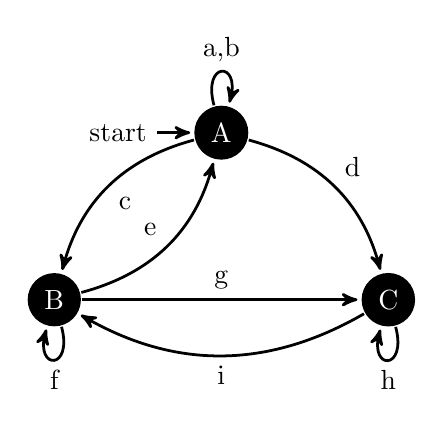
\begin{tikzpicture}[->,>=stealth',shorten >=1pt,auto,node distance=3cm,thick, line width = 1pt]
  \tikzstyle{every state}=[fill=black,draw=none,text=white,minimum size = 0.4cm]

{\node[state,initial]	(A)			{A};}
  
{\node[state]		(B) [below left of=A] 	{B};}
  
{\node[state]		(C) [below right of=A] 	{C};}


\path	(A) edge  [loop above] 	node {a,b} (A)
            edge  [bend right]	node {c} (B)
	    edge  [bend left]	node {d} (C)

        (B) edge [loop below] 	node {f} (B)
	    edge 		node {g} (C)
	    edge [bend right]	node {e} (A)
	
	(C) edge [loop below] 	node {h} (C)
	    edge [bend left] 	node {i} (B)
% 	    edge [bend left]	node {f} (A)
	 ;            
\end{tikzpicture}

%
%\caption{asdfadfs}


%\caption{Robot that does a DFS on binary trees.}
%\label{fig:dfs}
%%\hfill
%%\begin{minipage}[b]{0.45\linewidth}
%%    \centering
%%    \input{butterfly}
%%    \caption{}
%%    \label{fig: butterfly}
%%\end{minipage}
%%
%%\begin{minipage}[b]{0.45\linewidth}
%%    \centering
%%    \input{eye}
%%    \caption{}
%%    \label{fig: eye}
%%\end{minipage}
%\end{figure}
%



\head{Robot Tasks.} \label{ex:tasks}
%
Robots should achieve some task in their environment.
%: a {\em $k$-robot task}, or simply a {\em task}, $\T$, is a function that maps a graph $G$ to a set of sequences of positions of $G$, i.e.,  $\T(G) \subseteq (V^k)^\omega$. A robot-ensemble $\tup{R}$ {\em achieves} $\T$ on $G$ if for every run $\alpha$ of $\tup{R}$ on $G$ it holds that $\alpha' \in \T(G)$, where $\alpha'$ is the sequence of positions of the run $\alpha$.
%%\sr{should define tasks to be properties of runs? i.e., include states}
%
We give some examples of foundational robot tasks \cite{KKR07handbook}:
%\item A robot {\em explores and halts} if, no matter where it starts, it a) eventually halts, and b) visits every vertex of the graph at least once.
%
%\item A robot {\em explores and returns} if, no matter where it starts, it a) eventually halts where it started, and b) visits every vertex of the graph at least once.
%Formally, $v_1 v_2 \cdots \in T(G)$ if and only if there exists $i$ such that $\{v_1,\cdots,v_i\} = V$ and for all $j \geq i$, $v_i = v_j$.
%\sr{but the robot does not know it halts. tasks should also talk about the sequence of states, not just sequence of positions?}
%\item[RT3.] A robot {\em perpetually explores} if, no matter where it starts, it visits every vertex of $G$ infinitely often.

 A robot ensemble {\em deploys} or {\em reconfigures} if they move, in a collision-free way, to a certain target configuration.

 A robot ensemble {\em gathers} if, no matter where each robot starts, there is a vertex $z$, such that eventually every robot is in $z$.

 A robot ensemble {\em collaboratively explores} a graph if, no matter where they start, every node is eventually visited by at least one robot.

All of these tasks have {\em safe} variations: the robots complete their task without entering certain pre-designated ``bad'' nodes.
%
%\item[RT4.] An ensemble of robots {\em catches} a single robot if no matter where they start, at some point in time one robot in the ensemble is in the same vertex as the single robot. Note that unlike the previous examples, this task is adversarial.
% A robot {\em explores} if, no matter where it starts, it eventually visits every vertex of the graph at least once.


%no space
%Note that there are some natural relations between these tasks. If robots can explore and return, then in particular they can explore and halt. If they can explore and halt, then they can perpetually explore. If they can perpetually explore then, using the fact that they have IDs, they can gather --- every robot searches for the robot with the smallest ID, which stays still (with two agents this is called ``wait for mommy'').


\head{Multi-Robot Task Logic --- \MRTL.} \label{sec:TL}
%
We now define \MRTL, a logic for formally expressing robot tasks. We first define the syntax and semantics, and then we give some example formulas.  Later (in Lemma \ref{lem:msodefinable}) we prove that, when restricted to bounded-switching orderings, \MRTL\ formulas (and therefore many interesting natural tasks) can be converted into $\msol$ formulas over graphs.


{\bf $\MRTL$ Syntax.} Fix $k \in \nat$ and $\Sigma$. Formulas of $\MRTL_k$ are built, as in the definition of $\msol(\Sigma)$ from Section~\ref{dfn:msol}, from the following atomic formulas: $x=y$, $edg_{\sigma}$ (for $\sigma \in \Sigma$), $x \in X$, $\true$, and the following \underline{additional atomic formulas}  (with free variables $\tup{X},\tup{x},\tup{y}$ each of size $k$)
$Reach_{Q}, Halt^K_{Q}, Infty_{Q}$ and $Rept^K_{Q}$ where $Q \in \{\exists,\forall\}$ and $\emptyset \neq K \subseteq [k]$.

{\bf $\MRTL$ Semantics.} Formulas of $\MRTL_k$ are interpreted over graphs $G$, and with respect to $k$-robot ensembles $\tup{R}$ and a set of orderings $\Omega$.
%Thus, given a graph $G$ and $k$-ensemble of robots $\tup{R}$ where the $i$th robot $R_i$ has state set $Q_i$, initial-state set $I_i$,
%% repeating-state set $A$,
%and halting-state set $H_i$, accepting-state set $A_i$,
Define the satisfaction relation $\models_{\tup{R},\Omega}$:
\begin{itemize}
\item $G \models_{\tup{R},\Omega} Reach_\exists(\tup{X},\tup{x},\tup{y})$ iff \fbox{there is} an ordering $\alpha \in \Omega$ and there is a finite run of $\tup{R}$ on $G$ that uses a schedule that follows $\alpha$, such that the run starts with some initial configuration of the form $\tpl{\tup{x},\tup{p}}$ (i.e., $\tup{p} \in \prod I_i$), ends with a configuration of the form $\tpl{\tup{y},\tup{q}}$ (i.e., $\tup{q} \in \prod Q_i$), and for each $i \in [k]$, the set of positions of robot $i$ on this run is contained in $X_i$.

\item $G \models_{\tup{R},\Omega}Halt^K_\exists(\tup{X},\tup{x},\tup{y})$ means the same as $Reach_\exists$ except that the last tuple of states $\tup{q}$ has the property that $i \in K$ implies that $q_i \in H_i$ (i.e., every robot in $K$ is in a halting state).

\item $G \models_{\tup{R},\Omega}Infty_\exists(\tup{X},\tup{x},\tup{y})$ means the same as $Reach_\exists$ except that the run is infinite and $\tup{y}$ is visited infinitely often.

\item $G \models_{\tup{R},\Omega}Rept^K_\exists(\tup{X},\tup{x},\tup{y})$ means the same as $Reach_\exists$ except that the run is infinite, and infinitely often it reaches a configuration of the form $\tpl{\tup{y},\tup{q}}$ such that $i \in K$ implies $q_i \in A_i$.\sr{note that this means that every robot in $K$ is infinitely often, and simultaneously, in an accepting state. what natural task can be expressed using this atom?}

\item $G \models_{\tup{R},\Omega}Reach_\forall(\tup{X},\tup{x},\tup{y})$ is the same as $Reach_\exists$ except replace ``there is an ordering $\alpha \in \Omega$ and there is a finite run...'' by ``\fbox{for every} ordering $\alpha \in \Omega$ {there is} a finite run ...''. In a similar was define $Halt^K_\forall, Infty_\forall$ and $Rept^K_\forall$.
\end{itemize}

Extend the satisfaction relation to all formulas of $\MRTL_k$ in the natural way.
Denote by $\MRTL$ the set of formulas $\cup_k \MRTL_k$.

\example{ 
 The statement
 $
 G \models_{\tup{R},\Omega}(\forall \tup{x}) (\exists \tup{y}) (\exists \tup{X}) Reach_{\exists}(\tup{X},\tup{x},\tup{y}) \wedge (\wedge_{i,j} y_i = y_j) 
 $
means that, no matter where the robots start in $G$, there is an ordering $\alpha \in \Omega$, and a run according to a schedule that follows $\alpha$, such that the robots $\tup{R}$ gather at some vertex of the graph $G$. Replacing $Reach_\exists$ by $Reach_\forall$ means, no matter where the robots start in $G$, for every ordering $\alpha \in \Omega$, the robots have a run according to a schedule that follows $\alpha$ such that the robots gather at a vertex of the graph. Note that by conjuncting with $\wedge_i X_i \cap B = \emptyset$ where $B$ is an $\msol$-definable set of ``bad'' vertices, one can express ``safe gathering''.}

\example{\label{ex:formulas}

%The statement
%$
%G \models_{\tup{R},\Omega}  (\forall \tup{x}) (\exists \tup{X}) Halt^{[k]}_{\exists}(\tup{X},\tup{x},\tup{x}) \wedge (\wedge_i X_i = V)
%$
% expresses that, no matter where they start, there is a run according to a schedule that follows some $\alpha \in \Omega$, so that each robot {explores and returns} to its original .

Consider the statement
$
G \models_{\tup{R},\Omega} (\forall \tup{x}) [\textsc{nonleaf}(\tup{x}) \wedge \textsc{diff}(\tup{x}) \to (\textsc{leaf}(\tup{y}) \wedge \textsc{diff}(\tup{y}) \wedge Reach_{\forall}(V^k,\tup{x},\tup{y})]
$
where $G$ is a tree, $\textsc{nonleaf}(\tup{x})$ is an $\msol$-formula expressing that every $x_i$ is not a leaf, $\textsc{leaf}(\tup{y})$ is an $\msol$-formula expressing that every $y_i$ is a leaf, and $\textsc{diff}(\tup{z})$ is an $\msol$-formula expressing that $z_i \neq z_j$ for $i \neq j$. The statement says that, as long as the robots start on different internal nodes of the tree $G$, for every ordering $\alpha \in \Omega$ there is a run of the robots $\tup{R}$ according to a schedule that follows $\alpha$ in which the robots {reconfigure} and arrive at different leaves.
}

%\item The $\msol$-formula $\forall \tup{x} \exists \tup{y} \exists \tup{X}. \bigcup X_i = V \wedge \psi_\alpha(\tup{X},\tup{x},\tup{y})$ says that, no matter where they start, there is a run according to a schedule that follows $\alpha$ in which the robots collaboratively explore the graph.

%\item The $\msol$-formula (to be interpreted on trees)
%where $\textsc{nonleaf}(\tup{x})$ is an $\msol$-formula expressing that every $x_i$ is not a leaf, $\textsc{leaf}(\tup{y})$ expresses that every $y_i$ is a leaf, and $\textsc{diff}(\tup{z})$ expresses that $z_i \neq z_j$ for $i \neq j$. On trees this formula expresses that for every ordering $\alpha$ of processes that switch $N$-times, there is a run according to a schedule that follows $\alpha$ such that the robots reconfigure from different internal nodes to different internal leaves.\footnote{If one wants to add that the paths of the robots are collision-free one can replace $Reach$, for the case of two robots in which robot $1$ moves and then robot $2$ moves (for instance), by the formula
%$\exists \tup{Z} \exists \tup{Y} \exists \tup{z}\left[ \psi_1(\tup{Z},\tup{x},\tup{z}) \wedge \psi_2(\tup{Y},\tup{z},\tup{y})
%  \wedge Z_1 \cap Y_2 = \emptyset \right]
%$.}

% expresses, on trees, that no matter which internal nodes of the tree two robots start on, they have a collision-free path ($Z_1 \cap Y_2 = \emptyset$) in which they reach different leaves, according to a schedule in which robot $1$ is scheduled and then robot $2$ is scheduled. Similar more complex formulas can express the reconfiguration task of Example \ref{ex:recon} for (collaborative or adversarial) $b$-switching schedules.
%\item The atomic formula $Infty(X,x,y)$ expresses that the robot, starting in position $x$, visits position $y$ infinitely often, and the set of vertices the robot visits along this run is exactly $X$. Thus $\forall x Infty(V,x,x)$ is an \MRTL\ formula expressing that the robot ``perpetually explores'' the graph.

%\item The \MRTL\ formula $\exists \tup{x} \exists \tup{X} [Halt(\tup{X},\tup{x},\tup{x}) \wedge \cup_i X_i = V ]$, which talks about $k$ robots, expresses that each robot eventually returns and halts in its starting position, and every vertex of the graph is visited by at least one of the robots.


%\item The atomic formula $Infty(X,x,y)$ expresses that the robot, starting in position $x$, visits position $y$ infinitely often, and the set of vertices the robot visits along this run is exactly $X$. Thus $\forall x Infty(V,x,x)$ is an \MRTL\ formula expressing that the robot ``perpetually explores'' the graph.

%\item The \MRTL\ formula $\exists \tup{x} \exists \tup{X} [Halt(\tup{X},\tup{x},\tup{x}) \wedge \cup_i X_i = V ]$, which talks about $k$ robots, expresses that each robot eventually returns and halts in its starting position, and every vertex of the graph is visited by at least one of the robots.

%if $k=1$ and Lemma~\ref{lem:kcompile} if $k > 1$;
%$Q := \prod_{i \in [k]} Q_i$ is the set of tuples of states, $I := \prod_{i \in [k]} I_i$ is the set of tuples of initial states, $A := \prod_{i \in [k]} A_i$ are the repeating tuples, and $H := \prod_{i\leq k} H_i$ are the halting tuples.  We will often supress mention of $k$ and write, for instance, $Reach(\tup{X},\tup{x},\tup{y})$.

%an execution $\alpha \in (V^k \times \prod_{i \in [k]} Q_i)^*$ with $\alpha_1$ an initial configuration suppose $I_i \subseteq Q_i$ are the initial states, $A_i \subseteq Q_i$ are the accepting states, and $H_i \subseteq Q_i$ are the halting states:
%$(G,\tup{R}) \models Reach(\tup{x},\tup{y})$ iff there exists a  &\textrm{ iff } \alpha_1 = (\tup{q},\tup{x}) \textrm{ is initial, and } \exists i \in \nat\, \alpha_i = \tup{y}$


% such and every $k$-robot ensemble $\tup{R} = \tpl{R_1,\cdots,R_k}$, and all $k$-tuples of states $\tup{q},\tup{s} \in \prod_{i \in [k]} Q_i$, there is an atomic formula $\tup{R}_{\tup{p},\tup{q}}$  (of arity $2k$) where $\tup{R}_{\tup{p},\tup{q}}(\tup{x},\tup{y})$ expresses that there is an execution of the ensemble $\tup{R}$ starting with configuration $\tpl{\tup{x},\tup{p}}$ and containing\sr{ending?} the configuration $\tpl{\tup{y},\tup{q}}$.


%Formulas written in MSOL can quantify over sets (of vertices and edges). Thus they can express graph properties such as whether the graph is connected, whether it has  a $k$-colouring, whether it is planar, but not whether it is rigid.\sr{are these relevant properties?}

%A cornerstone of automata theory states that MSOL over finite/infinite words/trees coincides with automata operating on finite/infinite words/trees \cite{}.
%MSOL
\vspace{-1mm}

\section{Reasoning about Robot Systems}
\vspace{-1mm}

We formalise the parameterised verification problem for robot protocols and then study its decidability.
%, show that it is undecidable already in some very restricted cases, and then describe a simple restriction on the orderings, namely bounded switching, that guarantees decidability, which we show by reducing to the validity problem of certain logics.
%
%\head{The Parameterised Verification Problem.}
The parameterised verification problem depends on a (typically infinite) set of graphs $\gclass$, a set of $k$-robot ensembles $\rclass$, a $k$-robot task written as an $\MRTL_k$ formula $\T$, and a set of $k$-orderings $\Omega$.

\begin{definition}
The \textbf{parameterised verification problem} $\PVP_{\T,\Omega}(\gclass,\rclass)$ is: given a robot ensemble $\tup{R}$ from $\rclass$, decide whether for every graph $G \in \gclass$, $G \models_{\tup{R},\Omega} \T$ (i.e., the robots $\tup{R}$ achieves the task $\T$ on $G$ with orderings restricted to $\Omega$).
\end{definition}

\begin{example}
Let $\gclass$ be the set of all binary trees, $\rclass$ be the set of all $k$-robot ensembles,  let $\Omega_b := \{\alpha \in [k]^* : ||\alpha|| = b\}$ be the set of {\em $b$-switch orderings}, and let $T$ be the task expressing that if the robots start on different internal nodes of a tree then they eventually reconfigure themselves to be on different leaves of the tree, no matter which ordering from $\Omega_b$ is chosen (cf. Example~\ref{ex:formulas}). We will see later that one can decide $\PVP_{\T,\Omega_b}(\gclass,\rclass)$ given $b \in \nat$. So, one can decide, given $b$, whether the protocol from the reconfiguration example (in the Introduction) succeeds for every ordering with $b$ switches.
\end{example}

In Section \ref{sec:PVPundec} we show that the PVP is undecidable even on lines, for simple tasks, and allowing the robots very restricted testing abilities, i.e., a robot can sense which of the other robots shares the same position with it, called ``local collision tests''.  In Section \ref{sec:PVPdec} we show that we can guarantee decidability merely by restricting the scheduling regime while allowing the robots full testing abilities, including testing positions and states of other robots ``remotely''.
% original text
%In \cite{BlHe67,Rubin15AAMAS} it is shown that the PVP is undecidable for two synchronous robots on a line, and very simple tasks. In light of this negative result, the next step is to explore in what ways can we restrict the robots to gain decidability. One possible direction is to limit the sensing/communication between the robots. Indeed, the above mentioned undecidability result assumes that each robot can sense/query whether the other robot is at the left-most position of the line. Another possibility is to consider the case of asynchronous robots. In Section \ref{sec:PVPundec} we show that the assumption of asynchronous robots alone does not guarantee decidability of the parameterised verification problem already in the very restricted case of reachability tasks on lines. Interestingly enough, our proof also applies to the synchronous case, and assumes only very limited sensing capabilities, namely, that a robot can sense which of the other robots shares the same position with it (i.e., ``collision detection''). This fact strongly suggests that limiting the robots' sensing capabilities may not be a very fruitful direction. In Section \ref{sec:PVPdec} we show that for asynchronous robots a suitable restriction on their scheduling regime guarantees decidability in many cases that are otherwise quite unrestricted with respect to the graphs explored, tasks to be performed, and the sensing capabilities of the robots.


\subsection{Undecidability of Multi-Robot Systems on a Line} \label{sec:PVPundec}
Our undecidability proof proceeds by reducing the halting problem of two counter machines to the parameterised verification problem. An \emph{input-free 2-counter machine} (2CM)~\cite{Minsky67} is a deterministic program manipulating two nonnegative integer counters using commands that can increment a counter by $1$, decrement a counter by $1$, and check whether a counter is equal to zero. We refer to the ``line numbers'' of the program code as the ``states'' of the machine. One of these states is called the \emph{halting state}, and once it is entered the machine \emph{halts}. Observe that a 2CM has a single computation, and that if it halts then the values of both counters are bounded by some integer $n$.
%
The \emph{non-halting problem for 2CMs} is to decide, given a 2CM $\cm$, whether it does not halt. This problem is known to be undecidable \cite{Minsky67}, and is usually a convenient choice for proving undecidability of problems concerning parameterised systems due to the simplicity of the operations of counter machines.

Let $\gclass$ be the set of all graphs that are finite lines. Formally, for every $n \in \nat$ there is a graph $L_n = (V_n,E_n,\Sigma,\lambda_n) \in \gclass$, where $\Sigma = \{l,r\}$, $V_n = [n]$, $E_n = \cup_{i < n} \{(i,i+1), (i+1,i)\}$, and the label $\lambda_n$ of an edge of the form $(i,i+1)$ is $r$, and of the form $(i+1,i)$ is $l$. We now describe how, given a 2CM $\cm$, one can construct a robot ensemble $\tup{R}$ which can, on long enough lines, simulate the computation of $\cm$.
Our robots have very limited sensing abilities: a robot can only sense if it at one of the two ends of the line or not, and it can sense which of the other robots are in the same node as it is (``collision detection''). Note that a robot does not know that another robot has collided with it (and then moved on) if it is not scheduled while they both occupy the same node.

The basic encoding uses two counter robots $\counter_1$ and $\counter_2$. The current position of $\counter_i$ on the line corresponds to the current value of counter $i$, and it moves to the right to increment counter $i$ and to the left to decrement it. Each of these robots also stores in its finite memory the current state of the 2CM. One difficulty with this basic encoding is how to ensure that the two counter robots always stay synchronised in the sense that they both agree on the next command to simulate, i.e., we need to prevent one of them from ``running ahead''. A second difficulty is how to update the state of the 2CM stored by a counter robot when it simulates a command that is a test for zero of the other counter. Note that both of these difficulties are very easy to overcome if one robot can remotely sense the state/position of the other robot.
%For example, the coordination can be achieved by the two robots taking turns by observing the parity of the other robot's state. However, since we are disallowing remote sensing of any kind, it is not immediately apparent that these difficulties can be overcome. As it turns out, they can be overcome even with the very limited sensing abilities that we allow.
Since we disallow such powerful sensing these difficulties become substantially harder to overcome. The basic idea used to overcome the first difficulty is to add synchronisation robots and have a counter robot move only if it has collided with the appropriate synchronization robot. Thus, by arranging that the synchronization robots collide with the counter robots in a round-robin way the latter alternate their simulation turns and are kept coordinated. In order to enforce this round-robin behavior we have to change the encoding such that only every other position on the line is used to encode the counter values. Thus, an increment or a decrement is simulated by a counter robot moving two steps (instead of one) in the correct direction. The basic ingredient in addressing the second difficulty is to add a {\em zero-test} robot that, whenever one counter is zero, moves to the position of the other counter's robot, thus signaling to it that the first counter is zero.

\begin{theorem} \label{thm:PVPundec}
For every 2CM $\cm$, there is a robot ensemble $\tup{R}$ which, for every $n \geq 5$, simulates on the line $L_n$ any prefix of the computation of $\cm$ in which the counters never exceed the value $(n-3)/2$.\sr{can we more clearly say what we mean by ``simulates''? }
\end{theorem}
\begin{proof}
The ensemble $\tup{R}$ consists of $9$ robots: the {\em counter} robots $\counter_0, \counter_1$, four {\em synchronisation} robots $\round_0,\round_1,\round_2,\round_3$, a {\em zero-test} robot $\zeroTest$, a {\em zero} robot $\zero$ that marks the zero position of the counters, and a {\em mover} robot $\mover$ whose role is to ensure that the robots can simulate more than one command of \cm\ only if their starting positions on the line are as in the {\em initialised configuration} escribed below ($(\ddagger)$). The value of a counter is encoded as half the distance between the corresponding counter robot and the $\zero$ robot (e.g., if $\zero$ is in node $3$ and $\counter_1$ is in node $7$ then the value of counter $1$ is $2$).


%The {\em position of a robot (at a point in time)} is its position measured from the left-end of the line.
$(\ddagger)$ ({\em initialised configuration}):
%Each robot is in a ``ready to simulate'' state, and their positions are as follows :
robots $\round_2, \round_3$ are in node $1$, robots $\round_0,\round_1$ are in node $2$, and the rest are in node $3$.

The definition of the transitions of the robots has the important property that there is only one possible run starting from the initialised configuration, i.e., at each point in time exactly one robot has a transition with a test that evaluates to $\true$. We assume that each robot remembers if it is at an odd or even node. This can be done even without looking at the node by storing the parity of the number of steps taken since the initialised configuration ($\ddagger$).

Each command of the 2CM $\cm$ is simulated by the ensemble using $4$ phases. For every $i \in \{0,1,2,3\}$, phase $i$ has the following internal stages: (1) the synchronization robots arrange themselves to signal to robot $\round_i$ that it can start moving to the right (this mechanism is described below $(\star)$). (2) robot $\round_i$ moves to the right until it collides with robot $\counter_j$ (where $j = i \bmod 2$). It is an invariant of the run that this collision is at an even node if $i$ is odd, and vice-versa. (3) robot $\counter_j$ moves one step to the left or to the right, in order to simulate the relevant half of the current command of $\cm$, as described below $(\dagger)$. (4) robot $\round_i$ moves to the right until it reaches the end of the line. Observe that if during this stage $\round_i$ collides with $\counter_j$ then (unlike stage 2) it is on a node with the same parity as $i$ (by the invariant, and since $\counter_j$ moved one step in stage 3). This parity information is used by $\counter_j$ to know that it should not move, and by $\round_i$ to know that it can continue moving to the right. (5) robot $\round_i$ moves to the left until it reaches the beginning of the line (see $(\star)$), which ends the phase (here, as in the previous stage, the parity information is used to ignore collisions with $\counter_j$). In case the other counter (i.e., counter $1-j$) is zero, stage (2) of phases $0,1$ are modified as follows: when robot $\round_i$ enters node $3$ from the left it collides with $\zero, \counter_{1-j}$ and $\zeroTest$; then, $\zeroTest$ and $\round_1$ move to the right together, where $\zeroTest$ always goes first, and then $\round_i$ follows in lock-step; at the end of stage $2$ both $\zeroTest$ and $\round_i$ collide with $\counter_j$, thus signalling to the latter that counter $1-j$ is zero. A similar modification to stages (4) and (5) makes $\zeroTest$ and $\round_i$ move in lock-step fashion all the way to the right and then back to the left depositing $\zeroTest$ back in node $3$.
%\sr{do we have to deal separately with the case that $\round_i$ and $\counter_i$ collide at the RHS?}
%
%Finally, in order to keep the robot $\boundary$ always to the right of the other robots at the beginning of every phase we modify stage (4) such that when $\round_i$ collides with $\boundary$ and it finds $\counter_j$ also there (this may occur if the latter moved right in the previous stage), then it is not allowed to move until $\boundary$ moves out of that node (which it does by stepping to the right).


$(\dagger)$: The operation performed by $\counter_j$ in stage (3) of each phase is as follows.
%Recall that we encode the value of a counter is half the distance between the corresponding counter robot and the $\zero$ robot.
In phase $0$ robot $\counter_0$ simulates the first half of the command, in phase $1$ robot $\counter_1$ simulates the first half of the same command, in phase $2$ robot $\counter_0$ simulates the second half of the command and in phase $3$ $\counter_1$ does so. For example, if the command is ``increment counter $0$'' then in phase $0$ robot $\counter_0$ moves right one step (and updates its simulated state of $\cm$ to be the next command of $\cm$), in phase $1$ robot $\counter_1$ moves right one step (and updates its simulated state of $\cm$), in phase $2$ robot $\counter_0$ moves again one step to the right (thus encoding an incremented counter), and in phase $3$ robot $\counter_0$ moves left one step (thus, returning to its previously encoded value). Simulating the other three increment and decrement commands is done similarly. The only other command we need to simulate is of the form ''if counter $i$ is zero goto state $p$ else goto state $q$''. Since this command does not change the value of any counter it is simulated by each counter robot going right in the first half of the simulation and left in the second half. The internal state of $\cm$ is updated to $p$ or $q$ depending on the value of the counter. When simulating the first half of the command, robot $\counter_j$ knows that counter $j$ (resp. $1-j$) is zero iff it sees $\zero$ (resp. $\zeroTest$) with it.

($\star$): We now show that every arrangement of the synchronization robots uniquely determines which one of them its turn it is to move. Let $\next(i) := i+1 \bmod 4, \prev(i) := i-1 \bmod 4$. An {\em initial arrangement for phase $i$} is of the following form: $\round_{\prev(\prev(i))}, \round_{\prev(i)}$ are in node $1$, and $\round_i, \round_{next(i)}$ are in node $2$. Note that the initialised configuration ($\ddagger$) contains the initial arrangement for phase $0$. We let the initial arrangement for phase $i$ signal that the next robot to move is $\round_{\prev(\prev(i))}$, which moves to the right, thus completing stage (1) of phase $i$. Hence, at the beginning of stage $2$ the arrangement is such that only $\round_{\prev(i)}$ is left in node $1$, which signals that $\round_i$ is the next robot to move, as needed for stage (2). Just before the end of stage (5), robot $\round_i$  returns to node $2$ from the left, and the above arrangement repeats itself. Hence, again it is $\round_i$ that moves, however, this time to the left (as indicated by its now different internal memory). The resulting arrangement at the end of phase $i$ is thus: $\round_{prev(i)}, \round_i$ are in node $1$ and $\round_{\next(i)}, \round_{\prev(\prev(i))}$ are in node $2$. Observe that this is exactly the initial arrangement for phase $\next(i)$, as required. Note that since robots have collision tests a robot can tell by sensing which other robots are with it (and which are not) exactly which arrangement of the ones described above it is in, and thus if it allowed to move or not.

% OTHER IDEA
%Finally, we describe how to amend the construction above to ensure that robots can only simulate the 2CM if they happen to begin in the initialised configuration ($\ddagger$), and otherwise the system deadlocks after a few steps without any robot entering a halting state.
%%Observe that when starting from the initialised configuration ($\ddagger$), the first three moves are always: $\round_2$ moves right, $\round_0$ moves right, $\counter_0$ moves right. Thus,
%We add the following guards: (i) $\round_2$ never moves if when first scheduled it sees that it is not on the left edge of the line, and the same goes for $\round_3$; (ii) $\counter_0$ never moves unless it sees all the robots (except $\round_1, \round_2, \round_3$) are with it when first scheduled; (iii) after making its first move, $\round_0$ never makes its second move unless $\zero$ is with it.
%It is not hard (though somewhat tedious) to see that these extra guards guarantee that if the robots do not start as specified in ($\ddagger$) then $\round_0$ will never be able to start moving right in phase $0$ of the simulation of the second command of $\cm$. By assuming w.l.o.g. that $\cm$ does not halt after one command we know that a faulty start can not lead to a simulation of a halting computation of $\cm$, as promised.


Finally, we describe how to amend the construction above by incorporating the robot $\mover$ to ensure that robots can only simulate the 2CM if they happen to begin in the initialised configuration ($\ddagger$), and otherwise the system deadlocks after a few steps without any robot entering a halting state.\footnote{One can modify the construction to remove the need for the $\mover$ robot, however we find the exposition with the $\mover$ clearer.}  Add to every transition of robot $\round_i$, for $i \in \{0,1,2,3\}$, the additional guard that $\mover$ is on the same node with it. Thus, $\mover$ enables the synchronisation robots to move, and if $\mover$ ever stops, then so does the simulation. Robot $\mover$ behaves as follows. It first verifies that the rest of the robots are in the initialised configuration by executing the following sequence (and stopping forever if any of the conditions in the sequence fail to hold): check that it is alone on the right-hand side of the line, move left until it collides with $\counter_0,\counter_1,\zero,\zeroTest$, move one step left and check that it collides with $\round_0,\round_1$, move one step left and check it is on the left-hand side of the line and collides with $\round_2,\round_3$. Once it verified that the robots are on the nodes specified by ($\ddagger$), it starts ``chasing after'' the currently active synchronisation robot, i.e., it remembers which robot is active and the direction it moves in, and moves in that direction (if it does not currently collide with that robot).\qed
\end{proof}

From the previous theorem we can easily deduce that $\cm$ halts iff there is a run of the ensemble $\tup{R}$ (on a long enough line, and that fully simulates the run of $\cm$) and in which the robots $\counter_0, \counter_1$ halt.  We thus get:
\begin{corollary}
Let $k = 9$, $\gclass$ be the set of lines, $\rclass$ the set of $k$-robot ensembles consisting of robots whose only tests are local collision tests and the ability to test the left (resp. right) end of the line, $\Omega$ the set of all $k$-orderings, and $\T$ the \MRTL\ formula  $(\forall \tup{x}) (\forall \tup{y}) (\forall \tup{X}) \neg Halt^{\{1\}}_\exists(\tup{X},\tup{x},\tup{y})$.\footnote{The formula expresses``for every initial configuration, and every scheduling of the robots, robot $1$ never enters a halting state''.}
 Then $\PVP_{\T,\Omega}(\gclass,\rclass)$ is undecidable.
\end{corollary}
Suitable modifications to the construction in the theorem yield that other tasks, such as ``certain robots gather'' or ``certain robots reconfigure'', are undecidable.

\begin{remark} \label{rem:synch}
Note that in the construction, starting from the initialised configuration, at most one robot can move at any time. Thus, allowing all robots that can act to act, as in the synchronous model, does not change anything. So, with minor modifications to deal with the initialisation phase, the theorem also holds for the synchronous model. This strengthens the previously known fact that the PVP is undecidable for synchronous robots on a line with remote testing abilities 
(i.e., robot $l$ can test if ``robots $i$ and $j$ are in the same node'') \cite{Rubin15AAMAS}.
\end{remark}

\subsection{Decidability of Multi-Robot Systems with Bounded Switching} \label{sec:PVPdec}
The previous section shows that decidability cannot be achieved in very limited situations. However, we now suggest a limitation on the {\em orderings} which guarantees decidability without requiring any other restrictions. Thus it works on many classes of graphs, robots, and tasks.
%
%\subsection{Reducing parameterised verification to logical validity} \label{subsec:reduc}
%As expected, there is a tradeoff between the various modeling choices.
%This will involve restricting the combination of $k, \T,\gclass$ and (the testing abilities of robots in) $\rclass$.
We first describe, at a high level, the approach we use to solve (restricted cases of) the parameterised verification problem $\PVP_{\T,\Omega}(\gclass,\rclass)$, cf. \cite{Rubin15AAMAS}.
Suppose we can build, for every $k$-ensemble $\tup{R}$ of robots, a formula $\phi_{\tup{R},\T,\Omega}$ such that for all graphs $G$ the following are equivalent:
i) $G \models \phi_{\tup{R},\T,\Omega}$ and ii)
 $\tup{R}$ achieves task $\T$ on $G$ with orderings restricted to $\Omega$.

Then, for every $\rclass$ and $\gclass$, we would have reduced the parameterised verification problem $\PVP_{\T,\mathcal{A}}(\gclass,\rclass)$ to the $\Phi_{\tup{R},\T,\mathcal{A}}$-validity problem for $\gclass$ where $\Phi_{\tup{R},\T}$ is the set of formulas $\{\phi_{\tup{R},\T,\mathcal{A}} : \tup{R} \in \rclass\}$. We now show how to build an $\msol$-formula
$\phi_{\tup{R},\T,\Omega}$ in case $\T$ is a formula of \MRTL\ and $\Omega$ is a finite set of finite orderings.
%\footnote{Note that in our approach $\phi_{\tup{R},T,\mathcal{A}}$ does not depend on $\rclass$ or on $\gclass$.}
%The {\em validity problem} for a set of formulas $\Phi$ (in the signature of graphs) is to decide, given $\phi \in \Phi$, whether every graph satisfies $\phi$.

We begin with a lemma that will be used as a building block. In the simplest setting the lemma says that for every $i \in [k]$ there is an $\msol$ formula with free variables $\tup{x},\tup{y}$ that holds on a graph $G$ if and only if robot $i$ can move in $G$ from $x_i$ to $y_i$ while all the other robots are frozen, i.e.,  $x_j = y_j$ for $j \neq i$.

%\begin{lemma}[$b$-active schedules] \label{lem:msodefinable}
%Fix $k$, and let $\tup{R}$ be a $k$-robot ensemble over instruction set $\ins_{\Sigma,k}$, and let
%$\tup{p}, \tup{q} \in \prod Q_i$ be $k$-tuples of states. For every $b \in \nat$
%one can effectively construct an $\msol(\Sigma)$ formula $\psi_{b,\tup{R},\tup{p},\tup{q}}$ with free variables $X_i,x_i,y_i$ ($i \in [k]$) such that for every graph $G$:  $G \models \psi_{b,\tup{R},\tup{p},\tup{q}}(\tup{X},\tup{x},\tup{y})$ if and only if there exists a run $c$ of $\tup{R}$ on $G$ starting from configuration $c_1 = \tpl{\tup{x},\tup{p}}$ according to some $b$-active schedule $A_1 A_2 \cdots$, that reaches, say at time $T$, the configuration $\tpl{\tup{y},\tup{q}}$, and such that
% \begin{itemize}
% \item for all $t \leq T$, configuration $c_t$ results from $c_{t-1}$ using actions $\ins_i$ for $i \in A_t$ such that $\ins_i$ does not test the position of robots in $A_i \setminus \{i\}$,
% \item for all $i \in [k]$, the set of positions of agent $i$ on the prefix $c_1 c_2 \cdots c_T$ is exactly $X_i$.
%\end{itemize}
%
%Similarly one can construct $\psi^\infty_{b,\tup{R},\tup{p},\tup{q}}(\tup{X},\tup{x},\tup{y})$ so that for every graph $G$: $G \models \psi^\infty_{b,\tup{R},\tup{p},\tup{q}}(\tup{X},\tup{x},\tup{y})$ if and only if there exists a run $c$ of $\tup{R}$ on $G$ starting from configuration $c_1 = \tpl{\tup{x},\tup{p}}$ according to some $b$-switching schedule $A_1 A_2 \cdots$ that reaches the configuration $\tpl{\tup{y},\tup{q}}$ infinitely often and the set of positions of robot $i$ on the run is exactly $X_i$ ($i \in [k]$).
%\end{lemma}

\begin{lemma}[From Robots to $\msol$] \label{lem:msodefinable}
Fix $k$, and let $\tup{R}$ be a $k$-robot ensemble over instruction set $\ins_{\Sigma,k}$.


For every $\tup{p}, \tup{q} \in \prod Q_i$ ($k$-tuples of states) and ordering $\alpha \in [k]^+$,
one can effectively construct an $\msol(\Sigma)$ formula $\psi_{\alpha,\tup{p},\tup{q}}(\tup{X},\tup{x},\tup{y})$ with free variables $X_i,x_i,y_i$ ($i \in [k]$) such that for every graph $G$: $G \models \psi_{\alpha,\tup{p},\tup{q}}(\tup{X},\tup{x},\tup{y})$ if and only if
 there exists a run $c$ of $\tup{R}$ on $G$ according to a schedule that follows $\alpha$, starting from configuration $c_1 = \tpl{\tup{x},\tup{p}}$ and reaching, for some $T \in \nat$, the configuration $c_T = \tpl{\tup{y},\tup{q}}$, such that for all $i \in [k]$, the set of positions of robot $i$ on the prefix $c_1 c_2 \cdots c_T$ is contained in $X_i$.


Similarly one can construct $\psi^\infty_{\alpha,\tup{p},\tup{q}}(\tup{X},\tup{x},\tup{y})$ so that for every graph $G$: $G \models \psi^\infty_{\alpha,\tup{p},\tup{q}}(\tup{X},\tup{x},\tup{y})$ if and only if there exists a run $c$ of $\tup{R}$ on $G$ according to a schedule that follows $\alpha$, starting from configuration $c_1 = \tpl{\tup{x},\tup{p}}$ and reaching the configuration $\tpl{\tup{y},\tup{q}}$ infinitely often, and such that the set of positions of robot $i$ on the run is contained in $X_i$ ($i \in [k]$).
\end{lemma}

\begin{proof}
Fix $k$ and $\tup{R}$.  We start with an auxiliary step. For $i \in [k]$, states $p_i, q_i \in Q_i$, and $\tup{s} = (s_1, \cdots, s_{i-1}, s_{i+1}, \cdots, s_k)$ with $s_j \in Q_j$,  we define an MSO-formula $\phi_{i,p_i,q_i,\tup{s}}$ with free variables $X,x,y,\tup{z}$ where $\tup{z} = (z_1, \cdots, z_{i-1}, z_{i+1}, \cdots, z_k)$ such that $G \models \phi_i$ if and only if the $k$-ensemble robot $\tup{R}$ has a run according to a schedule in $i^*$ in which robot $i$ starts in position $x$ and state $p_i$, and reaches position $y$ and state $q_i$ while only visiting vertices in $X$, and for $j \neq i$, robot $j$  is in vertex $z_j$ and state $s_j$ and does not move or change state. This is done as follows. Each robot $R_i = \tpl{Q_i,\delta_i}$ is a finite automaton (without initial or final states) over a finite alphabet $Alph$ of instructions.
%, i.e., $Alph \subset \{\tau \to \kappa: \tau \in \msol_k(\Sigma), \kappa \in \{\uparrow_\sigma : \sigma \in \Sigma\} \cup \{\circlearrowleft\}\}$. 
By Kleene's theorem we can build a regular expression $exp_i$ (that depends on $p_i,q_i,\tup{s}$) over $Alph$ for the language of the automaton $R_i$ with initial state $p_i$ and final state $q_i$.
%
By induction on the regular expressions we build $\msol$ formulas (with free variables $X,x,y,\tup{z}$):
\begin{itemize}
\item $\varphi_{\emptyset} := \false$;
\item $\varphi_{\epsilon} := x = y \wedge x \in X$,
\item if $\tau \in \msol_k(\Sigma)$ is a position-test then
\begin{itemize}
\item[--] $\varphi_{\tau \to \uparrow_\sigma} := \tau(z_1,\cdots, z_{i-1},x,z_{i+1},\cdots,z_k) \wedge edg_\sigma(x,y) \wedge x,y \in X$,
\item[--] $\varphi_{\tau \to \circlearrowleft} :=  \tau(z_1,\cdots, z_{i-1},x,z_{i+1},\cdots,z_k) \wedge x = y \wedge x \in X$,
\end{itemize}
\item if $\tau$ is a state-test, say ``robot $j$ is in state $l$'' (for $j \neq i$ and $l \in Q_j$) then, if $s_j = l$ then
\begin{itemize}
\item[--] $\varphi_{\rho \to \uparrow_\sigma} :=  edg_\sigma(x,y) \wedge x,y \in X$,
\item[--] $\varphi_{\rho \to \circlearrowleft} :=   x = y \wedge x \in X$,
\end{itemize}
and otherwise if $s_j \neq l$, then $\varphi_{\rho \to \uparrow_\sigma}$ and $\varphi_{\rho \to \circlearrowleft}$ are defined to be $\false$,
\item $\varphi_{r + s} := \varphi_{r} \vee \varphi_{s}$,
\item $\varphi_{r \cdot s} := \exists w \left[\varphi_{r}(X,x,w,\tup{z}) \wedge \varphi_{s}(X,w,y,\tup{z})\right]$,
\item $\varphi_{r^*} := \forall Z [(cl_{\varphi_r}(X,Z,\tup{z}) \wedge x \in Z) \to y \in Z]$ where
$cl_{\varphi_r}(X,Z,\tup{z})$ is defined as $\forall a,b \left[(a \in Z \wedge \varphi_r(X,a,b,\tup{z})) \to b \in Z\right]$.

\end{itemize}

Then, define $\phi_{i,p_i,q_i,\tup{s}}$ to be $\varphi_{exp_i}(X,x,y,\tup{z})$.
%
% no space
%Note that for the Kleene-star we use the fact that $1$-ary transitive-closure with parameters is definable in MSO (as in Example MF4 in Section~\ref{sec:prelim}).
%Note that one can similarly find a formula $\phi_i^\infty$ 	that expresses that robot $i$ reaches $y$ infinitely often (starting in $x$ and visiting exactly the vertices in $X$) while the other robots do not move or change state.
%
%
To prove the lemma proceed by induction on the length $l$ of $\alpha$.
%
Base case: For $\alpha = i \in [k]$, define $\psi_{i,\tup{p},\tup{q}}(\tup{X},\tup{x},\tup{y})$ by
$
\bigwedge_{j \neq i} x_j = y_j \wedge X_j = \{x_j\}
\wedge \phi_{i,p_i,q_i,\tup{s}}(X_i,x_i,y_i,x_1, \cdots, x_{i-1}, x_{i+1}, \cdots, x_k)
$
if $\tup{s} = (p_1, \cdots, p_{i-1}, p_{i+1}, \cdots, p_k)$ and $q_j = s_j$ for $j \neq i$ (otherwise the formula is defined as $\false$).
%
Inductive case: For $\alpha \in [k]^+, i \in [k]$, define $\psi_{\alpha \cdot i,\tup{p},\tup{q}}(\tup{X},\tup{x},\tup{y})$ by
$
 \exists \tup{z}  \bigvee_{\tup{r}} \left[ \psi_{\alpha,\tup{p},\tup{r}}(\tup{X},\tup{x},\tup{z}) \wedge \psi_{i,\tup{r},\tup{q}} (\tup{X},\tup{z},\tup{y})\right]
$
 and $\tup{r}$ varies over $\prod Q_i$.
This completes the construction of $\psi_\alpha$.  The construction of $\psi^\infty_\alpha$ is similar.
%no space
% define
%$\psi^\infty_i$ to be like $\psi_i$ except replace $\phi_i$ by $\phi_i^\infty$,
%and define $\psi^\infty_{\alpha \cdot i}$ to be
%\[
% \exists \tup{Z} \exists \tup{Y} \exists \tup{z}\left[ \psi_\alpha(\tup{Z},\tup{x},\tup{z}) \wedge \psi_i^\infty(\tup{Y},\tup{z},\tup{y})
%  \wedge \bigwedge_{j \leq k} (X_j = Y_j \cup Z_j)\right]
%\]
%which expresses that the run first follows a schedule follows $\alpha$ and then robot $i$ is scheduled forever and position $\tup{y}$ is seen infinitely often.\qed
\qed
\end{proof}

In Lemma~\ref{lem:msodefinable}, a variable $X_i$ designates a set containing
-- but not necessarily equal to -- the positions of robot $i$ along the run.
% (i.e., if $\psi_{\alpha,\tup{p},\tup{q}}(\tup{X},\tup{x},\tup{y})$ is true for $X_i$ then it is also true for any set that contains $X_i$). 
If one wishes $X_i$ to designate the exact set of positions
visited by robot $i$ (in order to express, e.g., ``exploration''),
then one needs to modify the construction of $\phi_{i,p_i,q_i,\tup{s}}$ in the proof of the
lemma.\footnote{In~\cite{Rubin15AAMAS} it is wrongly stated that one can transform an
$\msol$ formula that says that there is a run (satisfying some property) that stays within a set
$X$, to one that says that it also visits all of $X$, by simply requiring that $X$ be a minimal
set for which a run satisfying the property exits.} The required modifications are
straightforward except for those to the definition of $\varphi_{r^*}$, which are more
complicated.\footnote{Recall that $\varphi_{r^*}$ has free variables $X,x,y,\tup{z}$, and its
semantic in this case is that robot $i$ can reach $y$ from $x$ (with the other robots' positions
being $\tup{z}$), visiting exactly $X$, using a concatenation of sub-paths each satisfying
$\varphi_{r}$. Intuitively, $\varphi_{r^*}$ existentially quantifies over
the stitching points of these sub-paths and uses appropriate sub-formulas that are all
satisfied iff one can find sub-paths that can be stitched to lead from $x$ to $y$ and that cover
all the positions in $X$.}

Observe that this lemma can be used to express both collaborative and adversarial scheduling.  For instance, if $\Omega$ is a finite set of orderings,
the formula
$
\bigvee_{\alpha \in \Omega} \psi_{\alpha,\tup{p},\tup{q}}(\tup{X},\tup{x},\tup{y})
$
says that there is an ordering $\alpha \in \Omega$ that the robots can follow to go from $\tup{x}$ to $\tup{y}$ while staying in $\tup{X}$, i.e., the ordering is chosen collaboratively. On the other hand, the formula
$
\bigwedge_{\alpha \in \Omega} \psi_{\alpha,\tup{p},\tup{q}}(\tup{X},\tup{x},\tup{y})
$
says that for every ordering $\alpha \in \Omega$, the robots can go from $\tup{x}$ to $\tup{y}$ while staying in $\tup{X}$, i.e., the ordering is chosen adversarially.


%\sr{TODO?: add result on slightly more general case in which some agents are frozen}

%
%\sr{proof of this lemma shows how to do a Kleene-star. Don't need TC for this, can just guess the set of stitching points. use the fact that if there is a word in $L^*$ then there is a short word that uses each stitching point once.}

%A more general lemma:
%\begin{lemma}[$b$-frozen schedules]
%For each $C \subseteq [k]$ one can effectively construct an $\msol(\Sigma)$ formula $\psi_{C,\tup{R},\tup{p},\tup{q}}$ with free variables $X_i,x_i,y_i$ ($i \in [k]$) such that for every graph $G$:  $G \models \psi_{C,\tup{R},\tup{p},\tup{q}}(\tup{X},\tup{x},\tup{y})$ if and only if there exists a run $c$ of $\tup{R}$ on $G$ starting from configuration $c_1 = \tpl{\tup{x},\tup{p}}$ according to some schedule $A_1 A_2 \cdots$, and a time $T \in \nat$ so that $c_T = \tpl{\tup{y},\tup{q}}$, and such that for all $t \leq T$,
%\begin{enumerate}
%\item $A_t \subseteq C$ (i.e., agents not in $C$ are frozen), and
%\item if $i \in A_t$ and the transition that robot $i$ takes from $c_t$ to $c_{t+1}$ is a test, say $\phi(z_1,\cdots,z_k)$, then $\phi$ does not mention the variables $z_j$ for $j \in C \setminus \{i\}$ (i.e., agent $i$ can only test its own position and the positions of agents not in $C$),
%\end{enumerate}
%and for all $i \in [k]$, the set of positions of agent $i$ on the prefix $c_1 c_2 \cdots c_T$ is exactly $X_i$.
%
%\end{lemma}

%BEGIN OLD
\iffalse
We now present a variation for $k > 1$. The argument mimics that in the proof of Lemma~\ref{lem:msodefinable}. However, the use of the transitive-closure operator is problematic because, as we stated in Example~\ref{ex:ktc} in the introduction, the $k$-ary transitive closure of an $\msol$-formula is not, in general, expressible in $\msol$.
Thus we make the additional assumption that each robot is star-free.

\begin{lemma} \label{lem:kcompile}
Let $\tup{R}$ be a $k$-robot ensemble, and let $\tup{p}, \tup{q} \in \prod Q_i$. Suppose that, for every $i \in [k]$, the language of instructions of automaton $R_i$ with initial state $p_i$ and final state $q_i$ is star-free.

We can build $\msol(\Sigma)$ formulas $\psi_{\tup{R},\tup{p},\tup{q}}$ so that for every graph $G$:
$G \models \psi_{\tup{R},\tup{p},\tup{q}}(\tup{X},\tup{x},\tup{y})$ if and only if the run of $\tup{R}$ on $G$ starting from configuration $\tpl{\tup{x},\tup{p}}$ has a prefix that reaches configuration $\tpl{\tup{y},\tup{q}}$ and the set of positions on the prefix of robot $i$ is exactly $X_i$ (for $i \in [k]$).

We can build $\msol(\Sigma)$ formulas $\psi^\infty_{\tup{R},\tup{p},\tup{q}}$ so that for every graph $G$: $G \models \psi_{\tup{R},\tup{p},\tup{q}}(\tup{X},\tup{x},\tup{y})$ if and only if the run of $\tup{R}$ on $G$ starting from configuration $\tpl{\tup{x},\tup{p}}$ reaches configuration $\tpl{\tup{y},\tup{q}}$ infinitely often and the set of positions on the run of robot $i$ is exactly $X_i$ (for $i \in [k]$).
\end{lemma}
%
\begin{proof}

First build the product automaton $\prod \tup{R}$ over alphabet $Alph \subset (\ins_{\Sigma,k})^k$: the state set $Q$ is $\prod_{i \in [k]} Q_i$,  and there is a transition from state $\tup{r}$ to state $\tup{s}$ with label $\tup{d} \in (\ins_{\Sigma,k})^k$ iff $(r_i,d_i,s_i) \in \delta_i$ for each $i \in [k]$. We claim that the language of $\prod \tup{R}$ with initial state $\tup{p}$ and final state $\tup{q}$ is star-free. This is an immediate consequence of the following general fact: if $W$ and $W'$ are star-free regular languages over alphabet $B$, then the product language $\{pair(w,w') : |w| = |w'|, w \in W, w' \in W'\}$ is star-free over alphabet $B\times B$, where $pair(w,w')$ is the word $(w_1, w'_1) (w_2,w'_2) \cdots$. To prove this fact use the McNaughton-Papert Theorem and its generalisation to $\omega$-words (discussed in Section~\ref{sec:prelim})  and the simple observation that given $\fol$-formulas $\phi$ defining $W$ and $\phi'$ defining $W'$,  the required $\fol$-sentence defining the product language can be taken as $\phi[P_b \gets \vee_{c\in B} P_{(b,c)}] \wedge \phi'[P_b \gets \vee_{c\in B} P_{(c,b)}]$.

Continue as in the proof of Lemma~\ref{lem:msodefinable}: induct on the star-free $\omega$-regular expression for $\prod \tup{R}$. The Kleene-star and $\omega$-power cases are skipped and we only need deal with the new complementation case. If $r$ is a star-free $\omega$-regular expression then the formula $\varphi_{\neg r}(\tup{X},\tup{x},\tup{y})$ is defined by eliminating negations by repeatedly using the following rules:
\begin{itemize}
\item $\varphi_{\neg \emptyset} := \varphi_{Alph^*}$
\item $\varphi_{\neg \epsilon} := \varphi_{Alph^+}$
\item $\varphi_{\neg \uparrow_\sigma} := $ \sr{FNISH!}
\item $\varphi_{\neg \tau} := \tup{x} = \tup{y} \wedge \neg \tau(\bar{x}) \wedge (\bigwedge_i x_i \in X_i)$.
\item $\phi_{\neg (r + s)} := \phi_{\neg r} \wedge \phi_{\neg s}$
\item $\phi_{\neg (r \cdot s)}(\tup{X},\tup{x},\tup{y})$ is defined as $\exists z. A \vee B \vee C$ where
\begin{align*}
A &:= \phi_{\neg r}(\tup{X},\tup{x},\tup{z}) \wedge \phi_{s}(\tup{X},\tup{z},\tup{y})\\
B &:= \phi_{\neg r}(\tup{X},\tup{x},\tup{z}) \wedge \phi_{\neg s}(\tup{X},\tup{z},\tup{y})\\
C &:= \phi_{r}(\tup{X},\tup{x},\tup{z}) \wedge \phi_{\neg s}(\tup{X},\tup{z},\tup{y}).
\end{align*}
\end{itemize}
One can check that $G \models \varphi_{\neg r}$ if and only if there is a sequence of instructions $ins \in Alph^*$ rejected  by the regular expression $r$ and a path from $\tup{x}$ to $\tup{y}$ that follows instructions $ins$, and that only visits vertices in $\tup{X}$.
\end{proof}
\fi
%END OLD



Putting everything together, we solve the PVP for finite sets of orderings (and thus for adversarial or co-operative $b$-switch orderings $\Omega_b := \{\alpha : ||\alpha|| = b\}$).

\begin{theorem} \label{thm:PVPdec}
There is an algorithm that given edge-label set $\Sigma$, a number of robots $k \in \nat$, a formula $\T$ of $\MRTL_k$, a finite set $\Omega$ of finite $k$-orderings, and a description of a context-free set of $\Sigma$-graphs $\gclass$, decides $\PVP_{\T,\Omega}(\gclass,\rclass)$, where  $\rclass$ is the set of all $k$-ensembles of robots over $\ins_{\Sigma,k}$.
%\footnote{Actually more is true: there is an algorithm that given $k \in \Nat, \Omega, \T$ and a description of $\gclass$ returns an algorithm that solves $\PVP_{\T,\Omega}(\gclass,\rclass)$ where $\rclass$ is the set of all $k$-ensembles of robots over $\ins_{\Sigma,k}$.}
\end{theorem}
%
\begin{proof}
Given $\tup{R} \in \rclass$ build the formula $\phi_{\tup{R},\T,\Omega}$ by replacing every atomic formula in
$\T$ by its definition with respect to $\tup{R}$. E.g., $Reach_\exists(\tup{X},\tup{x},\tup{y})$ is replaced by
$
\bigvee_{\alpha \in \Omega} \bigwedge_{\tup{p}} \bigvee_{\tup{q}} \psi_{\alpha,\tup{p},\tup{q}} (\tup{X},\tup{x},\tup{y}),
$
where $\tup{p}$ varies over $\prod_{i  \in [k]} I_i$ and $\tup{q}$ varies over $\prod_{i \in [k]} Q_i$.
%
Now, a routine induction on the structure of the formula $\T$ shows that $G \models_{\tup{R},\Omega} \T$ if and only if $G \models \phi_{\tup{R},\T,\Omega}$. By Lemma \ref{lem:msodefinable} the formula $\phi_{\tup{R},\T,\Omega}$ is in $\msol(\Sigma)$. Finally, apply the fact that the $\msol$-validity problem for context-free sets of graphs $\gclass$ is uniformly decidable \cite{CE12}. \qed
\end{proof}

%Consider the following extension of the model in which robots can {\em communicate their local state}. A robot can test the current state of another robot, i.e., it has a test ``robot $a$ in state $q$'' that is true if and only if the current state of Robot $j$ is $q$.
%
%\begin{theorem}
%Fix an edge-label set $\Sigma$, a number of robots $k \in \nat$, a set $\rclass$ of $k$-ensembles of robots that can also test the current states of other robots, a formula $\T$ of $\MRTL_k$, and a finite set $\Omega$ of finite orderings. If $\gclass$ is a context-free set of $\Sigma$-graphs, then $\PVP_{\T,\Omega}(\gclass,\rclass)$ is decidable.
%\end{theorem}
%
%\begin{proof}[Sketch]
%We show how to reduce the verification of robots with communication to robots without this ability, so that Theorem \ref{thm:PVPdec} can then be applied.
%
% Given $\tup{R} \in \rclass$. Suppose the states of the robots are from the set $Q = \{1,2,\cdots,N\}$.
%
%Transform graph $G$ to a graph $G_Q$ as follows: The domain of $G_Q$ is $G \times Q$; if $(g,h) \in E$ is labeled $\sigma$, then for all $i,j \in Q$ there is an edge from $(g,i)$ to $(h,j)$ labeled $(\sigma,j)$; and for every $g \in V, i, j \in Q$ there is an edge from $(g,i)$ to $(g,j)$ labeled $(\circlearrowleft,j)$ (thus we overload the symbol $\circlearrowleft$ and use it as part of graph labels). Further, label each vertex $(g,i)$ by a colour $i$ (formally we add unary-predicates $col_i$ to $\Sigma$-graphs).
%
%Transform robot $R \in \tup{R}$ to a robot $R_Q$  as follows: replace the test ``robot $a$ in state $i$''  by the ordinary test (i.e., $\msol$-formula) expressing that the colour of the position of robot $a$ is $i$; replace every transition of the robot of the form $(i,\tau \to \kappa, j)$ by the transition $(i,\tau \to (\kappa,j),j)$.
%
%Transform $\T$ to $\T'$ by replacing the atoms and relativising the quantifiers as follows. Define an equivalence relation $\equiv$ on $G \times Q$ by $x \equiv y$ :if $edg_{(\circlearrowleft,j)}(x,y) \wedge col_i(y)$. Define $\sqsubseteq$ on sets: $X \sqsubset Y$ if for every $x \in X$ there is a $y \in Y$ such that $x \equiv y$. Define $X \equiv Y$ by $X \sqsubseteq Y \wedge Y \sqsubseteq X$.
%Define a transformation of formulas $\phi \mapsto \phi_Q$ inductively as follows:
%\begin{itemize}
%\item $(x = y)_Q := x \equiv y$ and $(X = Y)_Q := X \equiv Y$.
%\item $(x \in Y)_Q := \exists z. z \equiv x \wedge z \in X$.
%\item $(edg_\sigma(x,y))_Q := \bigvee_j edg_{(\sigma,j)}(x,y)$.
%\item $(Reach_\exists(\tup{X},\tup{x},\tup{y}))_Q$ is defined to be
%\[
%\bigvee_{\alpha \in \Omega} \bigwedge_{\tup{p}} \bigvee_{\tup{q}} \left[ \psi_{\alpha,\tup{R},\tup{p},\tup{q}} (\tup{X},\tup{x},\tup{y}) \wedge (\wedge_i col_{p_i}(x_i)) \wedge (\wedge_i col_{q_i}(y_i)) \right]
%\]
%where $\tup{p}$ varies over $\prod_{i  \in [k]} I_i$ and $\tup{q}$ varies over $\prod_{i \in [k]} Q_i$. Transformations of the other atoms are defined similarly.
%\item $(\phi \wedge \psi)_Q := \phi_Q \wedge \psi_Q$, and $(\neg \phi)_Q := \neg \phi_Q$,
%\item $(\forall x. \phi(x,-))_Q := (\forall x) (\exists z \equiv x) \phi_Q(z,-)$ and $(\forall X. \phi(X,-))_Q := (\forall X) (\exists Z \equiv X) \phi_Q(Z,-)$.
%\end{itemize}
%
%Claim: $\tpl{G,\tup{R},\Omega} \models \T$ if and only if $\tpl{G_Q,\tup{R_Q},\Omega} \models \T_Q$.
%
%Finally, use the fact that there is an algorithm that given $Q$ and $\msol$-formula $\phi$ decides whether every $G \in G_Q$ satisfies $\phi$. Such an algorithm exists since for every $Q$ the set of graphs $\gclass_Q := \{G_Q : G \in \gclass\}$ is effectively context-free, i.e., there is an algorithm that given $Q$ and an $\msol$-sentence defining $\gclass$ produces an $\msol$-sentence defining $\gclass_Q$. This is due to the fact that $G \mapsto G_Q$ can be expressed by an $\msol$-transduction, and the image of a context-free set of graphs by an $\msol$-transduction is again context-free \cite{CE12}. \qed
%\end{proof}

%BEGIN OLD
\iffalse
\begin{theorem} \label{thm:PVPdec}
Fix $k \in \nat$ and edge-label set $\Sigma$. Let $\rclass$ be the set of all robots over $\ins_{\Sigma,1}$ if $k=1$, and all star-free $k$-robot ensembles over $\ins_{\Sigma,k}$ if $k > 1$. Let $\T$ be a $k$-robot task that is captured by an \MRTL\ formula, and let $\gclass$ be a set of $\Sigma$-graphs with decidable $\msol$-validity problem. Then $\PVP_\T(\gclass,\rclass)$ is decidable.
\end{theorem}
%
\begin{proof}
Say \MRTL\ formula $\vartheta$ captures $\T$. Given $\tup{R} \in \rclass$, build the formula $\phi_{\tup{R},\T}$ by replacing every atomic formula in $\vartheta$ by its definition with respect to $\tup{R}$, e.g., $Reach(\tup{X},\tup{x},\tup{y})$ is replaced by $\bigwedge_{\tup{p} \in I} \bigvee_{\tup{q} \in Q} \psi_{\tup{R},\tup{p},\tup{q}}(\tup{X},\tup{x},\tup{y})$. A routine induction on the structure of the formula $\vartheta$ gives: $\tpl{G,\tup{R}} \models_\MRTL \vartheta$ if and only if $G \models \phi_{\tup{R},\T}$. But by Lemma~\ref{lem:msodefinable} (or Lemma~\ref{lem:kcompile} if $k > 1$), $\phi_{\tup{R},\T}$ is a formula in $\msol(\Sigma)$. Thus we can apply the fact that the $\msol$-validity problem for $\gclass$ is decidable to decide whether $G \models \phi_{\tup{R},\T}$ for all $G \in \gclass$.
\end{proof}
\fi
%END OLD

%
%\begin{note} \label{note:thm2} Suppose, in Lemma~\ref{lem:kcompile}, one deletes the phrases ``the set of positions on the prefix/run is exactly $X_i$'',  and that test instructions are assumed to be $\mathcal{L}$-formulas, for $\mathcal{L} = \fol(\Sigma)$ or $\mathcal{L} =\fotc(\Sigma)$. Then the promised formulas $\psi_{\tup{R},\tup{p},\tup{q}}(\tup{x},\tup{y})$ and $ \psi_{\tup{R},\tup{p},\tup{q}}^\infty(\tup{x},\tup{y})$ are $\mathcal{L}$-formulas.
%Thus, suppose that $\T$ is definable in the fragment of $\MRTL$ that uses these ``set-less'' formulas. If, in addition, all robots are star-free, then to conclude that $\PVP_\T(\gclass,\rclass)$ is decidable, it is enough that $\gclass$ have decidable $\mathcal{L}$-validity problem.
%\end{note}
%

\vspace{-1mm}

\section{Discussion}
\vspace{-1mm}

In \cite{BlHe67,Rubin15AAMAS} (see also the discussion before Theorem \ref{thm:PVPundec}) it was shown that the PVP is undecidable for two synchronous robots on a line, reachability tasks, and allowing the robots ``remote'' position-tests. In Section \ref{sec:PVPundec} we refine this result and prove that the problem is still undecidable even if we only allow robots ``local'' position-tests or even just local ``collision tests''. The fact that the proof works for both the synchronous and asynchronous models (Remark \ref{rem:synch}), strongly suggests that limiting the robots' sensing capabilities may not be a very fruitful direction for decidability. In Section \ref{sec:PVPdec} we showed that for asynchronous robots, if one imposes a bound on the number of times the robots can switch, then PVP is decidable for very general tasks (i.e., those expressible in a new logic called \MRTL), large classes of graphs (i.e., the context-free sets of graphs), and allowing robots very powerful testing abilities (i.e., $\msol$ position-tests {\em and} state-tests). This is the first parameterised decidability result of the PVP for {\em multiple} robots where the environment is the parameter. Thus, our work indicates that if practitioners want formal guarantees on the correctness of the robot protocols they design, then they could design them in the framework given in this paper (i.e., finite-state, bounded-switching, powerful testing abilities).

The main limitation of our decidability result is the fact that the set of grids is not context-free --- grids are the canonical workspaces since they abstract 2D and 3D real-world scenarios.  However, this limitation is inherent and not confined to our formalisation since the parameterised verification problem even for one robot ($k=1$) on a grid with only ``local'' tests is undecidable \cite{BlHe67,Rubin15AAMAS}. A second limitation is that robots do not have a rich memory (e.g., they cannot remember a map of where they have visited). Extending the abilities to allow for richer memory and communication will result in undecidability, unless it is done in a careful way. Also, the complexity of the decision procedure we gave is very high. Again this is inherent in the problem since, e.g., already for one robot on trees the PVP with the ``explore and halt'' task is \exptime-complete \cite{Rubin15AAMAS}.  We leave for future research the problem of finding decidability results with reasonable complexity for multi-robot systems that are rich enough to capture protocols found in the distributed computing literature, e.g., \cite{BeSl95,KKR06,FPS11,FPS12}.
%\item Survey on the rendezvous task \cite{KKR06}
%\item Two deterministic robots with local traffic report can rendezvous in undirected graphs \cite{BeSl95}

\bibliographystyle{abbrv}
\bibliography{lit-mc}
%\newpage
%\subsection{appendix to undecidability proof}

We now explain why the simulation of each instruction of $\cm$ is done in four
phases. First, observe that
if we dispense with the synchronization robots and allow the counter robots to
move freely then there is no way to ensure that the two counter robots are
coordinated. This may lead to a situation where one counter robot has simulated
more instructions than the other, rendering it impossible for it to simulate a
test for zero of the other counter (since the other counter robot encodes a
value that belongs to another point in time). As we later explain, the fact that
a counter robot cannot do anything unless one of its two synchronizing robots
collides with it, together with the fact that the synchronizing robots seek
their counter robots in alternation, ensures that the counter robots remain
coordinated. But first we argue why the naive approach using only two
synchronizing robots (and thus two phases), with the value of a counter encoded
by the distance of the counter robot from $\zero$ (instead of half that
distance), does not work. Consider for example the case where a single
synchronizing robot collides with a counter robot that proceeds to simulate a
decrement by going one step to the left. Unfortunately, when the synchronizing
robot goes left on its way back to the beginning of the line (to signal the
synchronizing robot of the other counter that it is its turn to move right) it
will again collide with the counter robot, which if scheduled can now go on and
simulate the next instruction of $\cm$, resulting in the same counter robot
simulating two (or even more) instructions without the other counter robot doing
anything, and thus losing coordination with it. By using $4$ synchronization
robots and $4$ phases we avoid this problem as follows.
Each counter robot and each synchronization robot remembers if it is in an odd
or even node (this is maintained by simply toggling an internal flag whenever it
moves one step in any direction). When robot $\counter_0$ is at an odd (resp.
even) node then it can move only if robot $\round_0$ (resp. $\round_2$) is on
the same node (the synchronizing robot on the other hand concludes that it
cannot move, thus ensuring that the counter robot is the only one that can
move), and it will move to an even (resp. odd) position. Similarly, when robot
$\counter_1$ is at an odd (resp. even) node then it can move only if robot
$\round_1$ (resp. $\round_3$) is on the same node, and it will move to an even
(resp. odd) position. Thus, for example, in phase $1$, after $\counter_0$ moves
following a collision with $\round_0$, when $\round_0$ collides with it again on
its way back left this does not enable $\counter_0$ to simulate another
instruction since it is now in an even node from which it can only move when
colliding with $\round_2$ (which will happen only in phase $3$), whereas
$\round_0$ is now able to continue moving since it detects that this collision
is in an even node (and not an odd one as in the first collision when it could
not move until $\counter_0$ moved away).

It is worth noting that the boundary robot $\boundary$ is not needed if one
wishes to allow the robots to detect when they have reached the right end of the
line. Note, however, that one cannot use the collision with the counter robot to
signal to the synchronization robot that it should start moving back left.
Indeed, when they collide the only available move is for the counter robot which
then moves away from the synchronizing robot, thus rendering this collision
effectively invisible from the latter.

We now turn to the role of the helper robots and the reason for stage (1) in
each phase. It is not hard to see that without the helper robots and stage (1)
at the beginning of each phase all the synchronization robots are in node $1$.
Thus, due to this symmetry, there is no way for them to know which phase should
start next (i.e., which of them should start moving to the right towards the counter robots). 
The helper robots allow us to break this symmetry, and their
distribution of the helper and synchronisation robots between nodes $1$ and $2$ serves to encode the current phase.

The way this is done is as follows:
At the start of phase $1$ robots $\round_0,\ldots,\round_3$ are on node $1$ and
robots $\helper_0,\ldots,\helper_3$ are on node $2$. When $\round_0$ sees that
$\round_1,\ldots,\round_3$ are with it then it moves right (from $1$ to $2$).
Then $\helper_0$ detects that all helper robots and $\round_0$ are with it and
it moves left from $2$ to $1$. Observe that at this point
$\helper_0,\round_1,\round_2,\round_3$ are on node $1$ and $\round_0, \helper_1,
\helper_2,\helper_3$ are on node $2$.
Now, detecting this configuration on node $1$, robot $\round_1$ moves right from
$1$ to $2$. This ends stage (1) of the first phase.
At this point $\round_0$ detects that it is on an even node (recall that a
synchronization robot remembers the parity of the node it is on) together with
$\round_1$ and starts stage (2) by moving right.
Recall that phase $1$ ends by $\round_0$ moving back all the way to the left
until it meets $\helper_0$ (and thus to node $1$). Thus, at the end of phase
$1$, robots $\round_0,\helper_0,\round_2,\round_3$ are on node $1$ and robots
$\round_1, \helper_1, \helper_2,\helper_3$ are on node $2$.
Phase $2$ starts by $\helper_0$ detecting this setup of node $1$ and moving
right to $2$, followed by $\helper_1$ detecting that all helper robots and
$\round_0$ are at $2$ and moving from $2$ to $1$.
At this point we have $\round_0,\helper_1,\round_2,\round_3$ are on node $1$ and
robots $\helper_0, \round_1, \helper_2,\helper_3$ are on node $2$. Observe that
this is this is a symmetric situation to the one we were in after the first two
moves in phase $1$, i.e., all the synchronizing robots are in node $1$ except
for the one whose index is the phase number minus $1$, and all the helper robots
are in node $2$ except for the one whose index is the phase number minus $1$.
Thus, we can now continue in a similar fashion as we did in phase $1$, by having
$\round_2$ detecting this configuration of node $1$ and moving right to node
$2$, etc. We continue in this fashion wrapping around in phase $4$, in which
after two steps we have that $\round_0,\round_1,\round_2, \helper_3$ are on node
$1$ and robots $\helper_0, \helper_1,\helper_2, \round_3$ are on node $2$, at
which point $\round_0$ detects this configuration of node $1$ and moves right to
node $2$, etc.



\end{document}

